\documentclass[12pt,a4paper]{article}
\usepackage[margin=2.2cm]{geometry}
\usepackage{ctex}
\usepackage{amsmath,amssymb,amsfonts}
\usepackage{graphicx}
\usepackage{tikz}
\usetikzlibrary{calc,positioning,arrows.meta,decorations.pathreplacing,matrix}
\usepackage{booktabs}
\usepackage{enumitem}
\usepackage{xcolor}
\usepackage{tcolorbox}
\usepackage{hyperref}
\usepackage{float}

\tcbuselibrary{theorems,skins,breakable}

\definecolor{myblue}{RGB}{0,102,204}
\definecolor{myred}{RGB}{204,0,0}
\definecolor{mygreen}{RGB}{0,153,0}
\definecolor{mypurple}{RGB}{128,0,128}
\definecolor{myorange}{RGB}{230,120,0}
\definecolor{lightblue}{RGB}{220,235,255}
\definecolor{lightyellow}{RGB}{255,255,220}
\definecolor{lightgreen}{RGB}{220,255,220}
\definecolor{lightred}{RGB}{255,225,225}

\newtcolorbox{keybox}[1][]{
  colback=lightblue, colframe=myblue,
  fonttitle=\bfseries, title={#1},
  breakable
}

\newtcolorbox{exbox}[1][]{
  colback=lightyellow, colframe=myorange,
  fonttitle=\bfseries, title={#1},
  breakable
}

\newtcolorbox{warnbox}[1][]{
  colback=lightred, colframe=myred,
  fonttitle=\bfseries, title={#1},
  breakable
}

\newtcolorbox{sumbox}[1][]{
  colback=lightgreen, colframe=mygreen,
  fonttitle=\bfseries, title={#1},
  breakable
}

\title{\Huge\textbf{MPS/MPO 张量网络方法详解} \\ \Large 以 N 皇后问题为例的完整教程}
\author{张量网络学习笔记}
\date{2026年3月}

\begin{document}

\maketitle
\tableofcontents
\newpage

%=============================================================================
\section{从零开始：什么是张量？}
%=============================================================================

\subsection{标量、向量、矩阵、张量}

\begin{keybox}[核心概念：张量的阶数]
\textbf{张量}就是多维数组，它的\textbf{阶数}（也叫\textbf{秩}）等于它有多少个指标（下标）。
\begin{itemize}
  \item \textbf{0 阶张量} = 标量（一个数）：$c = 3.14$
  \item \textbf{1 阶张量} = 向量（一列数）：$v_i$，如 $v = (1, 0, 1)$
  \item \textbf{2 阶张量} = 矩阵（一张表）：$M_{ij}$，如 $\begin{pmatrix} 1 & 0 \\ 0 & 1 \end{pmatrix}$
  \item \textbf{3 阶张量}：$T_{ijk}$，一个"立方体"的数
  \item \textbf{$n$ 阶张量}：$T_{i_1 i_2 \cdots i_n}$，$n$ 个指标
\end{itemize}
\end{keybox}

\begin{exbox}[例子：3 阶张量]
一个形状为 $[2,3,2]$ 的 3 阶张量 $T_{ijk}$：
\begin{itemize}
  \item 第 1 个指标 $i$ 取值 $\{1,2\}$（维度 2）
  \item 第 2 个指标 $j$ 取值 $\{1,2,3\}$（维度 3）
  \item 第 3 个指标 $k$ 取值 $\{1,2\}$（维度 2）
  \item 总共有 $2 \times 3 \times 2 = 12$ 个元素
\end{itemize}
你可以把它想象成 2 张 $3 \times 2$ 的表格叠在一起。
\end{exbox}

\subsection{张量的图形表示}

在张量网络领域，我们用\textbf{图形}来表示张量，规则非常简单：

\begin{keybox}[图形规则]
\begin{itemize}
  \item 一个张量 = 一个\textbf{节点}（圆圈或方块）
  \item 每个指标 = 从节点伸出的一条\textbf{线}（称为"腿"，leg）
  \item 线的维度 = 这个指标可以取多少个值
\end{itemize}
\end{keybox}

\begin{center}
\begin{tikzpicture}[scale=1.0]
  % Scalar
  \node[draw, circle, fill=myblue!20, minimum size=0.8cm] (s) at (0,0) {$c$};
  \node[below=0.3cm] at (s) {标量：0条腿};

  % Vector
  \node[draw, circle, fill=myblue!20, minimum size=0.8cm] (v) at (3,0) {$v$};
  \draw[thick] (v) -- ++(0,-1) node[below]{$i$};
  \node[below=1.3cm] at (v) {向量：1条腿};

  % Matrix
  \node[draw, circle, fill=myblue!20, minimum size=0.8cm] (m) at (6,0) {$M$};
  \draw[thick] (m) -- ++(-1,0) node[left]{$i$};
  \draw[thick] (m) -- ++(1,0) node[right]{$j$};
  \node[below=0.3cm] at (m) {矩阵：2条腿};

  % 3-tensor
  \node[draw, circle, fill=myblue!20, minimum size=0.8cm] (t) at (10,0) {$T$};
  \draw[thick] (t) -- ++(-1,0) node[left]{$i$};
  \draw[thick] (t) -- ++(1,0) node[right]{$k$};
  \draw[thick] (t) -- ++(0,-1) node[below]{$j$};
  \node[below=1.3cm] at (t) {3阶张量：3条腿};
\end{tikzpicture}
\end{center}

%=============================================================================
\section{张量缩并：最核心的运算}
%=============================================================================

\subsection{什么是缩并}

\begin{keybox}[张量缩并 = 广义的矩阵乘法]
两个张量\textbf{缩并}（contraction），就是把它们\textbf{共享的指标求和}。

矩阵乘法 $C_{ik} = \sum_j A_{ij} B_{jk}$ 就是最简单的缩并：对共享指标 $j$ 求和。
\end{keybox}

\begin{exbox}[例子1：矩阵乘法就是缩并]
设 $A$ 是 $2 \times 3$ 矩阵，$B$ 是 $3 \times 4$ 矩阵：
$$C_{ik} = \sum_{j=1}^{3} A_{ij} B_{jk}$$
图形表示：把 $A$ 的右腿和 $B$ 的左腿\textbf{连起来}。

\begin{center}
\begin{tikzpicture}[scale=1.0]
  % Before
  \node at (-1, 0.7) {\textbf{缩并前:}};
  \node[draw, circle, fill=myblue!20, minimum size=0.8cm] (a) at (0,0) {$A$};
  \draw[thick] (a) -- ++(-1,0) node[left]{$i$};
  \draw[thick,myred] (a) -- ++(1,0) node[right]{$j$};

  \node[draw, circle, fill=mygreen!20, minimum size=0.8cm] (b) at (3,0) {$B$};
  \draw[thick,myred] (b) -- ++(-1,0) node[left]{$j$};
  \draw[thick] (b) -- ++(1,0) node[right]{$k$};

  % Arrow
  \draw[-{Stealth}, thick] (5,0) -- (6,0);

  % After
  \node at (6.5, 0.7) {\textbf{缩并后:}};
  \node[draw, circle, fill=mypurple!20, minimum size=0.8cm] (c) at (8,0) {$C$};
  \draw[thick] (c) -- ++(-1,0) node[left]{$i$};
  \draw[thick] (c) -- ++(1,0) node[right]{$k$};
\end{tikzpicture}
\end{center}

红色的 $j$ 指标被求和掉了，只剩下 $i$ 和 $k$。结果 $C$ 是 $2 \times 4$ 矩阵。
\end{exbox}

\begin{exbox}[例子2：向量内积]
$$s = \sum_{i=1}^{n} u_i v_i = \mathbf{u} \cdot \mathbf{v}$$
两个向量各有 1 条腿，缩并后 0 条腿 $\to$ 标量。

\begin{center}
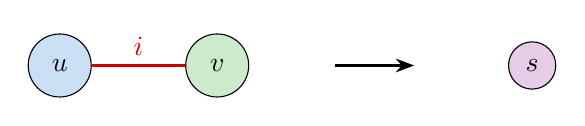
\begin{tikzpicture}
  \node[draw, circle, fill=myblue!20, minimum size=0.8cm] (u) at (0,0) {$u$};
  \node[draw, circle, fill=mygreen!20, minimum size=0.8cm] (v) at (2,0) {$v$};
  \draw[thick,myred] (u) -- (v) node[midway,above]{$i$};
  \draw[-{Stealth}, thick] (3.5,0) -- (4.5,0);
  \node[draw, circle, fill=mypurple!20, minimum size=0.6cm] (s) at (6,0) {$s$};
\end{tikzpicture}
\end{center}
\end{exbox}

\begin{exbox}[例子3：高阶张量缩并]
设 $A_{ijkl}$（4 阶）和 $B_{kmp}$（3 阶），对 $k$ 缩并：
$$C_{ijlmp} = \sum_{k} A_{ijkl} \, B_{kmp}$$
结果是 5 阶张量（4 + 3 - 2 = 5）。

\textbf{规则：每缩并一对指标，总腿数减 2。}
\end{exbox}

\subsection{图形上的缩并：连线 = 求和}

\begin{sumbox}[核心规则]
在张量网络图中：
\begin{itemize}
  \item \textbf{悬空的腿}（自由指标）= 结果张量的指标
  \item \textbf{两个节点之间的连线}（内部指标）= 被求和的指标
  \item 连线的维度 = 求和的范围
\end{itemize}
\end{sumbox}


%=============================================================================
\section{N 皇后问题：从棋盘到张量网络}
%=============================================================================

\subsection{N 皇后问题回顾}

在 $N \times N$ 的棋盘上放 $N$ 个皇后，使得：
\begin{itemize}
  \item 每\textbf{行}恰好 1 个皇后
  \item 每\textbf{列}恰好 1 个皇后
  \item 每条\textbf{对角线}最多 1 个皇后
\end{itemize}

问：有多少种合法的放法？

\subsection{关键思想：把约束变成张量}

\begin{keybox}[核心映射]
\begin{enumerate}
  \item 棋盘的每个格子 $(i,j)$ 放一个张量 $T_{i,j}$
  \item 张量的指标沿 8 个方向（上、下、左、右、四个对角）传递"\textbf{攻击信号}"
  \item 每个格子有一个状态 $p$：$p=1$（空）或 $p=2$（有皇后）
  \item 张量的非零元素编码了 \textbf{局部约束}：如果这里有皇后，就必须向所有方向发出攻击信号
  \item 将所有张量缩并起来（对所有内部指标求和），得到的标量就是\textbf{合法配置的总数}
\end{enumerate}
\end{keybox}

这和统计力学中的配分函数完全类似：
$$Z_N = \sum_{\text{所有配置}} \prod_{\text{所有格点}} W_{\text{格点}}$$
只不过权重 $W$ 对合法配置 = 1，非法配置 = 0。

\subsection{核心张量 B 的 9 个指标}

代码中定义的张量 $B$ 有 9 个指标，每个维度为 2：
$$B(u,\, ul,\, l,\, ld,\, d,\, dr,\, r,\, ru,\, p)$$

\begin{center}
\begin{tikzpicture}[scale=1.2]
  \node[draw, rectangle, fill=myblue!20, minimum size=1.2cm, rounded corners] (B) at (0,0) {$B$};

  % 8 directions
  \draw[thick,myred] (B) -- ++(0,1.2) node[above]{$u$ (上)};
  \draw[thick,myred] (B) -- ++(0,-1.2) node[below]{$d$ (下)};
  \draw[thick,myblue] (B) -- ++(-1.2,0) node[left]{$l$ (左)};
  \draw[thick,myblue] (B) -- ++(1.2,0) node[right]{$r$ (右)};
  \draw[thick,mygreen] (B) -- ++(0.9,0.9) node[above right]{$ru$ (右上)};
  \draw[thick,mygreen] (B) -- ++(-0.9,-0.9) node[below left]{$ld$ (左下)};
  \draw[thick,mypurple] (B) -- ++(-0.9,0.9) node[above left]{$ul$ (左上)};
  \draw[thick,mypurple] (B) -- ++(0.9,-0.9) node[below right]{$dr$ (右下)};

  % Physical index
  \draw[thick,myorange,dashed] (B) -- ++(1.5,-0.8) node[right]{$p$ (占据状态)};
\end{tikzpicture}
\end{center}

\begin{keybox}[每个指标的含义（维度都是 2）]
\begin{itemize}
  \item $u, d, l, r$：上、下、左、右方向的\textbf{列/行攻击信号}
  \item $ul, dr$：左上$\to$右下对角线的攻击信号
  \item $ur, ld$：右上$\to$左下对角线的攻击信号（代码中 $ru$ 和 $ld$）
  \item $p$：该格的\textbf{占据状态}（1=空，2=有皇后）
\end{itemize}

每个指标取值的意义：
\begin{itemize}
  \item 值 = 1：\textbf{该方向没有攻击信号}经过
  \item 值 = 2：\textbf{该方向有攻击信号}经过（该方向已经有一个皇后在攻击）
\end{itemize}
\end{keybox}

\subsection{B 张量非零元素的完整解读}

$B$ 总共 $2^9 = 512$ 个元素，其中只有 16 个非零（= 1），其余都是 0。每个非零元素对应一种\textbf{合法的局部状态}。

\subsubsection{情况一：格子为空（$p=1$），无皇后经过}

$$B(1,1,1,1,1,1,1,1,\;1) = 1$$

意思：所有方向都没有攻击信号，这个格子是空的。完全合法。

\subsubsection{情况二：格子为空（$p=1$），有信号"透传"}

当格子为空时，对角线上的攻击信号可以\textbf{穿过}这个格子。但规则是：
\begin{itemize}
  \item 对角线信号必须\textbf{成对出现}：从一边进，从另一边出
  \item 例如：左上有信号进来 ($ul=2$)，就必须从右下出去 ($dr=2$)
  \item 列/行信号同理：上面有信号 ($u=2$)，就必须向下传 ($d=2$)
\end{itemize}

\begin{exbox}[透传的例子]
$$B(2,1,1,1,2,1,1,1,\;1) = 1 \quad \text{列攻击信号：上→下透传}$$
意思：上方有皇后在这一列攻击 ($u=2$)，信号向下传递 ($d=2$)，这个空格子只是把信号传下去。

$$B(1,2,1,1,1,2,1,1,\;1) = 1 \quad \text{↘对角线信号：左上→右下透传}$$
意思：左上方对角线有皇后 ($ul=2$)，信号沿对角线向右下传 ($dr=2$)。

还有多条信号同时透传的情况：
$$B(2,2,1,1,2,2,1,1,\;1) = 1 \quad \text{列 + ↘对角线同时透传}$$
$$B(2,2,2,1,2,2,2,1,\;1) = 1 \quad \text{列 + ↘对角线 + ↗对角线同时透传（3条信号）}$$
\end{exbox}

透传规则总结（$p=1$ 时）：
\begin{center}
\begin{tabular}{ccc}
\toprule
\textbf{入方向} & \textbf{出方向} & \textbf{含义} \\
\midrule
$u=2$ & $d=2$ & 列攻击 \\
$ul=2$ & $dr=2$ & $\searrow$ 对角线 \\
$l=2$ & $r=2$ & 行攻击 \\
$ld=2$ & $ru=2$ & $\nearrow$ 对角线 \\
\bottomrule
\end{tabular}
\end{center}

这 4 条通道相互独立，每条可以开（2）或关（1），所以空格子有 $2^4 = 16$ 种可能。但其中 $p=2$（有皇后）的情况要另算，实际 $p=1$ 的合法状态有 $2^4 = 16$ 种——不过等等，当 $p=1$ 时还有一个 $B(1,1,1,1,2,2,2,2,\;2)$ 是 $p=2$ 的情况。

让我重新梳理：$p=1$（空格子）的非零元素是上面列出的 $2^4 - 1 = 15$ 个透传组合（选择哪些通道开），一共 $2^4 = 16$ 种（包括全关）。但代码中 $B$ 的最后一个指标是 $p$，我们看到：

$p=1$ 时有 15 个非零元素（0 到 4 条信号透传的各种组合）。

\subsubsection{情况三：格子有皇后（$p=2$）}

$$B(1,1,1,1,2,2,2,2,\;2) = 1$$

意思：这里放了一个皇后！它\textbf{没有}从任何方向接收攻击信号（$u=1, ul=1, l=1, ld=1$），但\textbf{向所有方向发出}攻击信号（$d=2, dr=2, r=2, ru=2$）。

\begin{warnbox}[为什么入方向都是 1？]
如果 $u=2$（上方同列已有皇后）同时 $p=2$（这里也有皇后），就\textbf{违反了列约束}！所以：
$$B(2,\cdot,\cdot,\cdot,\cdot,\cdot,\cdot,\cdot,\;2) = 0 \quad (\text{只要 } u=2 \text{ 且 } p=2)$$
类似地，如果任何入方向有攻击信号且这里有皇后，$B=0$。

\textbf{唯一合法的有皇后状态}：所有入方向都无信号 (=1)，所有出方向都有信号 (=2)。
\end{warnbox}

\subsubsection{为什么只有 16 个非零元素}

\begin{sumbox}[16 个非零元素 = 15（空格子透传）+ 1（放皇后）]
\begin{enumerate}
  \item 空格子 ($p=1$)：4 条独立通道，每条开/关 → $2^4 = 16$ 种（但 $B(2,2,2,2,2,2,2,2,1)=1$ 是全开的情况，代码中确实列出了）

  实际上代码中 $p=1$ 的非零元素：
  \begin{itemize}
    \item 0 条通道开：1 个（全 1）
    \item 1 条通道开：$\binom{4}{1} = 4$ 个
    \item 2 条通道开：$\binom{4}{2} = 6$ 个
    \item 3 条通道开：$\binom{4}{3} = 4$ 个
    \item 4 条通道开：$0$ 个？
  \end{itemize}

  等等，让我重新数。看代码：$B(2,2,2,2,2,2,2,2,\;1) = 1$，这是 4 条全开且 $p=1$（空格子），意思是这个空格子上所有四个方向都有攻击线经过——完全合法，只是不能放皇后。

  所以 $p=1$ 有 $1 + 4 + 6 + 4 + 1 = 16$ 个。但这加上 $p=2$ 的 1 个是 17 个？

  让我重数代码... 代码中明确列出的是：
  \begin{itemize}
    \item 行 4：$B(1,1,1,1,1,1,1,1,1)=1$
    \item 行 5：$B(2,2,2,2,2,2,2,2,1)=1$（4 条全开，$p=1$）
    \item 行 7-10：4 个单通道
    \item 行 12-17：6 个双通道
    \item 行 19-22：4 个三通道
    \item 行 24：$B(1,1,1,1,2,2,2,2,2)=1$（$p=2$，放皇后）
  \end{itemize}
  总计 $1+1+4+6+4+1 = 17$？不对，$1+4+6+4+1 = 16$ 个 $p=1$，加上 $1$ 个 $p=2$ = $17$ 个。

  但标题说 16 个... 让我再数一下代码中 B 的非零元素：第 4,5,7,8,9,10,12,13,14,15,16,17,19,20,21,22,24 行，共 17 行赋值。
\end{enumerate}

总结：$B$ 张量共 $17$ 个非零元素 = $16$（空格子的各种透传组合）+ $1$（放皇后）。
\end{sumbox}

\subsection{一个极简例子：$2\times 2$ 的情况}

\begin{exbox}[$2 \times 2$ 棋盘，理解信号传播]
$2\times 2$ 棋盘只有 4 个格子。N=2 皇后问题要在 $2\times 2$ 棋盘上放 2 个皇后使互不攻击——显然\textbf{无解}（$Z_2 = 0$）。

用张量网络来验证：如果在 $(1,1)$ 放皇后，它会向右发出行攻击信号（到 $(1,2)$），向下发出列攻击信号（到 $(2,1)$），向右下发出对角线信号（到 $(2,2)$）。这三个格子全部被封锁，无法放第二个皇后。其他位置同理。
\end{exbox}


%=============================================================================
\section{从 9 阶张量到 2D 网络张量：辅助张量的作用}
%=============================================================================

\subsection{问题：对角线指标如何处理？}

原始的 $B$ 张量有 9 个指标（8 个方向 + 1 个占据状态）。在正方格点上：
\begin{itemize}
  \item 上下左右 4 个方向的连接很自然（连到邻居格点）
  \item 但\textbf{对角线}方向呢？$(i,j)$ 的右下邻居是 $(i+1, j+1)$，不是直接的上下左右邻居
\end{itemize}

\begin{center}
\begin{tikzpicture}[scale=1.5]
  \node[draw, circle, fill=myblue!20, minimum size=0.6cm] (11) at (0,1) {\tiny$(1,1)$};
  \node[draw, circle, fill=myblue!20, minimum size=0.6cm] (12) at (1,1) {\tiny$(1,2)$};
  \node[draw, circle, fill=myblue!20, minimum size=0.6cm] (21) at (0,0) {\tiny$(2,1)$};
  \node[draw, circle, fill=myblue!20, minimum size=0.6cm] (22) at (1,0) {\tiny$(2,2)$};

  % Horizontal
  \draw[thick,myblue] (11) -- (12);
  \draw[thick,myblue] (21) -- (22);
  % Vertical
  \draw[thick,myred] (11) -- (21);
  \draw[thick,myred] (12) -- (22);
  % Diagonal - problem!
  \draw[thick,mygreen,dashed] (11) -- (22) node[midway,right]{\small\color{mygreen} 对角线？};
\end{tikzpicture}
\end{center}

对角线连接会让网络变成非平面的，无法用简单的 MPS/MPO 方法处理。

\subsection{解决方案概述：用 UE、DE、V0 把对角线变成上下左右}

代码的巧妙之处是引入了三个\textbf{辅助张量}：
\begin{itemize}
  \item \textbf{UE}：把对角线信号\textbf{编码}（合并）进垂直和水平键
  \item \textbf{DE}：把合并后的键\textbf{解码}（拆分）回独立的对角线信号
  \item \textbf{V0}：对占据状态 $p$ 求和（追踪所有配置）
\end{itemize}

其目标是：\textbf{消除所有对角线连接}，使张量网络变成纯粹的正方格子（只有上下左右的键），从而可以用 MPS/MPO 方法处理。

%------------------------------------------------------------
\subsection{UE 张量详解：对角线信号的编码器}

\subsubsection{第一步：4 维 SWAP 张量}

UE 最初定义为一个 4 阶张量，每个指标维度为 2：
$$\text{UE}(a, b, c, d) = \delta_{a,d} \cdot \delta_{b,c}$$

写出全部 $2^4 = 16$ 个元素，只有 4 个非零：

\begin{center}
\begin{tabular}{cccc|c|l}
\toprule
$a$ & $b$ & $c$ & $d$ & UE 值 & 含义 \\
\midrule
1 & 1 & 1 & 1 & \textbf{1} & $\delta_{1,1}\delta_{1,1}$：两对都匹配 \\
1 & 2 & 2 & 1 & \textbf{1} & $\delta_{1,1}\delta_{2,2}$：$a{=}d{=}1$，$b{=}c{=}2$ \\
2 & 1 & 1 & 2 & \textbf{1} & $\delta_{2,2}\delta_{1,1}$：$a{=}d{=}2$，$b{=}c{=}1$ \\
2 & 2 & 2 & 2 & \textbf{1} & $\delta_{2,2}\delta_{2,2}$：两对都匹配 \\
\bottomrule
\end{tabular}
\end{center}

\begin{keybox}[UE 的本质：SWAP 门]
UE 做的事情是：
$$\text{输入} (a, b) \to \text{输出} (c, d) = (b, a)$$
它\textbf{交换}两个指标。$\delta_{a,d}$ 保证 $d=a$（第一个输入 = 第二个输出），$\delta_{b,c}$ 保证 $c=b$（第二个输入 = 第一个输出）。

\begin{center}
\begin{tikzpicture}[scale=1.0]
  \draw[thick,myred] (0,1) node[left]{$a$} -- (2,0) node[right]{$d=a$};
  \draw[thick,myblue] (0,0) node[left]{$b$} -- (2,1) node[right]{$c=b$};
  \fill[white] (1,0.5) circle(0.15);
  \node at (1,-0.8) {SWAP：两条线交叉};
\end{tikzpicture}
\end{center}
\end{keybox}

\subsubsection{第二步：Reshape 为 $[2, 2, 4]$}

代码将 UE 的后两个指标 $(c, d)$ 合并为一个维度-4 的指标 $k$：
$$\text{UE}_r(a, b, k) \quad \text{其中} \quad k = c + 2(d - 1)$$

这是 MATLAB 的列优先（column-major）排列。映射表：

\begin{center}
\begin{tabular}{cc|c|l}
\toprule
$c$ & $d$ & 合并后 $k$ & 物理含义 \\
\midrule
1 & 1 & 1 & 两条对角线都无信号 \\
2 & 1 & 2 & $c$ 方向有信号，$d$ 方向无 \\
1 & 2 & 3 & $c$ 方向无信号，$d$ 方向有 \\
2 & 2 & 4 & 两条对角线都有信号 \\
\bottomrule
\end{tabular}
\end{center}

Reshape 后的 4 个非零元素：

\begin{center}
\begin{tabular}{ccc|c|l}
\toprule
$a$ & $b$ & $k$ & $\text{UE}_r$ & 来源 \\
\midrule
1 & 1 & 1 & \textbf{1} & $(c{=}1,d{=}1) \to k{=}1$ \\
1 & 2 & 2 & \textbf{1} & $(c{=}2,d{=}1) \to k{=}2$ \\
2 & 1 & 3 & \textbf{1} & $(c{=}1,d{=}2) \to k{=}3$ \\
2 & 2 & 4 & \textbf{1} & $(c{=}2,d{=}2) \to k{=}4$ \\
\bottomrule
\end{tabular}
\end{center}

\subsubsection{UE 的作用方式}

在 ncon 缩并中，UE 的三个指标分别连接到：
\begin{itemize}
  \item \textbf{指标 $a$}（dim 2）：与原始张量的 $dr$（右下对角线）缩并
  \item \textbf{指标 $b$}（dim 2）：输出到\textbf{水平键}（向右传递）
  \item \textbf{指标 $k$}（dim 4）：输出到\textbf{垂直键}（向下传递）
\end{itemize}

\begin{center}
\begin{tikzpicture}[scale=1.2]
  \node[draw, rectangle, fill=myorange!30, minimum width=1.5cm, minimum height=1cm, rounded corners] (ue) at (0,0) {UE};
  \draw[thick,myred,-{Stealth}] (-2,0) -- (ue.west) node[midway,above]{$a = dr$};
  \draw[thick,myblue,-{Stealth}] (ue.east) -- (2,0) node[midway,above]{$b$ → 水平键};
  \draw[thick,mygreen,-{Stealth}] (ue.south) -- (0,-1.2) node[below]{$k$ → 垂直键（dim 4）};
  \node[above=0.3cm] at (ue.north) {\small 输入：$dr$ 信号};
  \node[right=0.3cm] at (2,0) {\small 输出到右邻居};
  \node[below=0.1cm] at (0,-1.2) {\small 输出到下邻居};
\end{tikzpicture}
\end{center}

\begin{exbox}[具体例子：当 $dr = 1$（无对角线信号）时]
UE$_r(1, b, k)$ 的非零元素：
\begin{itemize}
  \item $(b{=}1, k{=}1)$：水平键输出 1（无信号），垂直键输出 1（无信号）
  \item $(b{=}2, k{=}2)$：水平键输出 2（有信号），垂直键输出 2
\end{itemize}

\textbf{为什么 $dr=1$ 却产生了两种输出？}

因为 UE 的 SWAP 结构要求 $d = a = dr$ 且 $c = b$。当 $dr = 1$ 时，$d$ 被固定为 1，但 $b$（和 $c=b$）是自由的。这意味着垂直键的 $k$ 中，$d$ 分量被锁定为 1，但 $c$ 分量可以取任何值——它携带的是\textbf{从其他位置传来的对角线信息}，与当前格点的 $dr$ 无关。

具体地：
\begin{itemize}
  \item $(b{=}1, k{=}1)$：对应 $(c{=}1, d{=}1)$ → 既无来自别处的信号，也无本格 $dr$ 信号
  \item $(b{=}2, k{=}2)$：对应 $(c{=}2, d{=}1)$ → 有来自别处的信号在传递，但本格 $dr$ 无信号
\end{itemize}
\end{exbox}

\begin{exbox}[具体例子：当 $dr = 2$（有对角线信号，这里有皇后！）时]
UE$_r(2, b, k)$ 的非零元素：
\begin{itemize}
  \item $(b{=}1, k{=}3)$：水平键 1，垂直键 3。对应 $(c{=}1, d{=}2)$：$dr$ 信号存入垂直键的 $d$ 分量
  \item $(b{=}2, k{=}4)$：水平键 2，垂直键 4。对应 $(c{=}2, d{=}2)$：$dr$ 信号 + 其他信号都有
\end{itemize}
\end{exbox}

\begin{warnbox}[UE 的关键特性：制造关联]
UE 使得水平键的值 $b$ 和垂直键的值 $k$ \textbf{不再独立}——它们通过 $c = b$ 的约束被关联起来。

这正是对角线约束被编码的方式：\textbf{对角线信号需要同时出现在水平和垂直方向}，UE 保证了这种一致性。

如果水平键传出了 $b=2$（有对角线信号），那么垂直键中 $c$ 分量也必须是 2——这意味着斜下方的邻居也能"看到"这个信号。
\end{warnbox}

%------------------------------------------------------------
\subsection{DE 张量详解：对角线信号的解码器}

\subsubsection{从单位矩阵出发}

$$\text{DE} = \text{reshape}(I_4, [4, 2, 2])$$

$I_4$ 是 $4 \times 4$ 单位矩阵。Reshape 后变成 3 阶张量，三个指标维度分别为 $(4, 2, 2)$。

$I_4$ 的非零元素在对角线上：$(1,1), (2,2), (3,3), (4,4)$。

MATLAB 列优先 reshape 的映射：$4 \times 4$ 矩阵的元素 $(\text{row}, \text{col})$ 对应线性索引 $\text{row} + 4(\text{col}-1)$，而 $[4,2,2]$ 张量的元素 $(k, i, j)$ 对应线性索引 $k + 4(i-1) + 8(j-1)$。

逐个计算 $I_4$ 对角线元素的映射：

\begin{center}
\begin{tabular}{c|c|ccc|l}
\toprule
$I_4$ 位置 & 线性索引 & $k$ & $i$ & $j$ & 含义 \\
\midrule
$(1,1)$ & 1 & 1 & 1 & 1 & $k{=}1$ → 双无，拆分为 $i{=}1, j{=}1$ \\
$(2,2)$ & 6 & 2 & 2 & 1 & $k{=}2$ → 拆分为 $i{=}2, j{=}1$ \\
$(3,3)$ & 11 & 3 & 1 & 2 & $k{=}3$ → 拆分为 $i{=}1, j{=}2$ \\
$(4,4)$ & 16 & 4 & 2 & 2 & $k{=}4$ → 双有，拆分为 $i{=}2, j{=}2$ \\
\bottomrule
\end{tabular}
\end{center}

\begin{exbox}[验证线性索引]
以 $I_4(2,2)$ 为例：线性索引 $= 2 + 4 \times (2-1) = 6$。

在 $[4,2,2]$ 张量中：$k + 4(i-1) + 8(j-1) = 6$，解得 $k=2, i=2, j=1$。\checkmark

以 $I_4(3,3)$ 为例：线性索引 $= 3 + 4 \times (3-1) = 11$。

在 $[4,2,2]$ 张量中：$11 - 8 = 3$，所以 $j=2$，剩下 $k + 4(i-1) = 3$，得 $k=3, i=1$。\checkmark
\end{exbox}

所以 DE 的 4 个非零元素是：

\begin{center}
\begin{tabular}{ccc|c}
\toprule
$k$ (dim 4) & $i$ (dim 2) & $j$ (dim 2) & DE 值 \\
\midrule
1 & 1 & 1 & \textbf{1} \\
2 & 2 & 1 & \textbf{1} \\
3 & 1 & 2 & \textbf{1} \\
4 & 2 & 2 & \textbf{1} \\
\bottomrule
\end{tabular}
\end{center}

\subsubsection{DE 的作用方式}

在 ncon 中，DE 的三个指标连接到：
\begin{itemize}
  \item \textbf{指标 $k$}（dim 4）：输入来自\textbf{垂直键}（从上方传来的合并信息）
  \item \textbf{指标 $i$}（dim 2）：与原始张量的 $ru$（右上对角线）缩并
  \item \textbf{指标 $j$}（dim 2）：输出到\textbf{水平键}（向右传递）
\end{itemize}

\begin{center}
\begin{tikzpicture}[scale=1.2]
  \node[draw, rectangle, fill=mygreen!30, minimum width=1.5cm, minimum height=1cm, rounded corners] (de) at (0,0) {DE};
  \draw[thick,mygreen,{Stealth}-] (0,1.2) -- (de.north) node[midway,right]{$k$ ← 垂直键（dim 4）};
  \draw[thick,myred,-{Stealth}] (de.south) -- (0,-1.0) node[below]{$i = ru$};
  \draw[thick,myblue,-{Stealth}] (de.east) -- (2,0) node[right]{$j$ → 水平键};
  \node[above=0.1cm] at (0,1.2) {\small 合并信号从上方来};
  \node[below=0.1cm] at (0,-1.0) {\small 拆出 $ru$ 对角线信号};
\end{tikzpicture}
\end{center}

\begin{exbox}[DE 的作用：拆分合并索引]
DE 做的恰好是 UE 的\textbf{逆操作}：

UE 把 $(c, d)$ 合并为 $k = c + 2(d-1)$，同时将 $b=c$ 和 $a=d$ 传出。

DE 把 $k$ 拆分回两个分量：
\begin{itemize}
  \item $k=1 \to (i{=}1, j{=}1)$：无信号
  \item $k=2 \to (i{=}2, j{=}1)$：$ru$ 方向有信号，$j$ 方向无
  \item $k=3 \to (i{=}1, j{=}2)$：$ru$ 方向无信号，$j$ 方向有信号（传给右邻居）
  \item $k=4 \to (i{=}2, j{=}2)$：两者都有信号
\end{itemize}

直觉：UE 是\textbf{编码器}（合并），DE 是\textbf{解码器}（拆分）。
\end{exbox}

%------------------------------------------------------------
\subsection{V0 张量：对占据状态求和}

$$V_0 = \begin{pmatrix} 1 \\ 1 \end{pmatrix} \quad \text{形状 } [2, 1]$$

V0 与原始张量的 $p$ 指标缩并：
$$\sum_{p=1}^{2} T(\ldots, p) \cdot V_0(p) = T(\ldots, 1) + T(\ldots, 2)$$

\textbf{效果}：把"空格子"和"有皇后"两种状态加起来。这正是配分函数的求和——我们要对所有可能的占据配置求和，让合法的贡献 1，非法的贡献 0。

%------------------------------------------------------------
\subsection{UE 与 DE 的协作：对角线信号的完整路由}

\begin{exbox}[完整路由例子：$(1,1)$ 的皇后攻击 $(2,2)$]
假设 $(1,1)$ 放了皇后，$dr = 2$。对角线信号如何到达 $(2,2)$？

\begin{center}
\begin{tikzpicture}[scale=1.3]
  % Grid
  \node[draw, rectangle, fill=myblue!20, minimum size=1.2cm, rounded corners] (t11) at (0,2) {$T_{1,1}$};
  \node[draw, rectangle, fill=white, minimum size=1.2cm, rounded corners] (t12) at (3,2) {$T_{1,2}$};
  \node[draw, rectangle, fill=white, minimum size=1.2cm, rounded corners] (t21) at (0,0) {$T_{2,1}$};
  \node[draw, rectangle, fill=myred!20, minimum size=1.2cm, rounded corners] (t22) at (3,0) {$T_{2,2}$};

  % Queen
  \node[above=0.1cm,myblue] at (t11.north) {\small 皇后};
  \node[below=0.1cm,myred] at (t22.south) {\small 被攻击};

  % Step 1: UE encodes dr into vertical bond
  \draw[very thick, mygreen, -{Stealth}] (t11.south) -- (t21.north)
    node[midway, left=0.3cm, text width=2.5cm, align=center]
    {\small\color{mygreen} 步骤1\\ UE 把 $dr{=}2$\\ 编码进垂直键\\ ($k=3$ 或 $4$)};

  % Step 2: DE extracts at T21, sends right
  \draw[very thick, myorange, -{Stealth}] (t21.east) -- (t22.west)
    node[midway, below=0.3cm, text width=3cm, align=center]
    {\small\color{myorange} 步骤2\\ DE 在 $T_{2,1}$ 处\\ 拆分，把信号\\ 转发到水平键};

  % Diagonal (what we want to achieve)
  \draw[thick, dashed, gray, -{Stealth}] (t11.south east) -- (t22.north west)
    node[midway, above right]{\small\color{gray} 对角线（被替代）};

  \draw[thick] (t11.east) -- (t12.west);
  \draw[thick] (t12.south) -- (t22.north);
  \draw[thick] (t21.east) -- (t22.west);
\end{tikzpicture}
\end{center}

\textbf{详细步骤}：
\begin{enumerate}
  \item 在 $T_{1,1}$：皇后使 $dr = 2$。UE 将 $a{=}dr{=}2$ 编码，产生 $k = 3$（当 $b{=}1$ 时）或 $k=4$（当 $b{=}2$ 时）。$k$ 通过垂直键传给 $T_{2,1}$。
  \item 在 $T_{2,1}$：DE 接收到 $k = 3$，拆分为 $(i{=}1, j{=}2)$。$j{=}2$ 通过水平键传给 $T_{2,2}$。$T_{2,2}$ 收到 $j{=}2$ 表示"有对角线攻击经过"，如果 $T_{2,2}$ 也想放皇后，就会因为入方向有信号而被 $B$ 张量的零元素封锁。
\end{enumerate}
\end{exbox}

\subsection{Reshape 后的键维度解读}

经过与 UE、DE、V0 缩并后，每个张量只剩 2-4 个指标，维度为 2、4 或 8：

\begin{keybox}[键维度的物理含义]
\begin{center}
\begin{tabular}{ccl}
\toprule
\textbf{维度} & \textbf{编码内容} & \textbf{举例} \\
\midrule
\textbf{2} & 1 条攻击线 & 角落处单条对角线 \\
\textbf{4} & 2 条攻击线 & 边缘处两条对角线 $(2\times 2)$ \\
\textbf{8} & 3 条攻击线 & 内部的列 + 两条对角线 $(2\times 2\times 2)$ \\
\bottomrule
\end{tabular}
\end{center}
\end{keybox}

\begin{exbox}[为什么内部垂直键维度是 8]
看内部张量 $B$ 的垂直键：它需要传递 3 种信号：
\begin{enumerate}
  \item \textbf{列攻击}：这一列上方/下方是否有皇后 → 1 bit（维度 2）
  \item \textbf{$\searrow$ 对角线}：经过这个键的下行对角线是否有皇后 → 1 bit（维度 2）
  \item \textbf{$\nearrow$ 对角线}：经过这个键的上行对角线是否有皇后 → 1 bit（维度 2）
\end{enumerate}
三者独立 → $2 \times 2 \times 2 = 8$。

具体地，垂直键的值 $\alpha \in \{1,2,\ldots,8\}$ 编码为三元组 $(c, d_1, d_2)$：
\begin{center}
\begin{tabular}{cccc}
\toprule
$\alpha$ & 列攻击 $c$ & $\searrow$ 对角线 $d_1$ & $\nearrow$ 对角线 $d_2$ \\
\midrule
1 & 无 & 无 & 无 \\
2 & 无 & 无 & 有 \\
3 & 无 & 有 & 无 \\
4 & 无 & 有 & 有 \\
5 & 有 & 无 & 无 \\
6 & 有 & 无 & 有 \\
7 & 有 & 有 & 无 \\
8 & 有 & 有 & 有 \\
\bottomrule
\end{tabular}
\end{center}
\end{exbox}

\begin{exbox}[为什么左右水平键维度有的是 4 有的是 8]
\textbf{水平键}需要传递的信号取决于它连接的是哪两列之间：
\begin{itemize}
  \item \textbf{第 1 行的水平键}（维度 4）：第 1 行上方没有格子，所以不需要传列信号（因为列信号是垂直的）。只需传两条对角线信息 → $2 \times 2 = 4$
  \item \textbf{内部行的水平键}（维度 8）：需要传递行攻击 + 两条经过的对角线信息 → $2 \times 2 \times 2 = 8$
  \item \textbf{右端边界键}（维度 2 或 4）：右边缘对角线更少
\end{itemize}
\end{exbox}


%=============================================================================
\section{完整数值推导：$T_{1,1}$ 的每一个元素}
%=============================================================================

下面以左上角 $T_{1,1}$ 为例，从头到尾追踪每一步缩并的数值，最终得到完整的 $8 \times 4$ 矩阵。

\subsection{第一步：原始 9 阶张量（2 个非零元素）}

$T_{1,1}$ 对应棋盘左上角（CLU），原始维度为：
$$T_{1,1}(u, ul, l, ld, d, dr, r, ru, p) \quad \text{形状 } [1,1,1,1,2,2,2,1,2]$$

边界效应：$u, ul, l, ld, ru$ 的维度都是 1（上方和左方没有邻居），所以这些指标被锁定为 1，只有 $d, dr, r, p$ 是自由的。

只有 \textbf{2} 个非零元素：

\begin{center}
\renewcommand{\arraystretch}{1.3}
\begin{tabular}{ccccccccc|c|l}
\toprule
$u$ & $ul$ & $l$ & $ld$ & $d$ & $dr$ & $r$ & $ru$ & $p$ & 值 & 物理含义 \\
\midrule
1 & 1 & 1 & 1 & 1 & 1 & 1 & 1 & 1 & \textbf{1} & 空格子，所有方向无信号 \\
1 & 1 & 1 & 1 & 2 & 2 & 2 & 1 & 2 & \textbf{1} & 放了皇后，向 $d,dr,r$ 发信号 \\
\bottomrule
\end{tabular}
\end{center}

\begin{warnbox}[为什么只有这 2 个？]
\begin{itemize}
  \item 这是\textbf{左上角}，上方和左方没有邻居 → 不可能有攻击信号从上方或左方进来
  \item 所以入方向 $u, ul, l, ld$ 全是 1
  \item 要么空（全 1），要么放皇后（$p{=}2$，向下 $d{=}2$、右下 $dr{=}2$、右 $r{=}2$ 发信号）
  \item $ru = 1$ 因为右上方没有邻居（这是第 1 行）
\end{itemize}
\end{warnbox}

\subsection{第二步：与 UE 缩并（$dr$ 信号编码）}

ncon 指令：
\begin{verbatim}
ncon({T{1,1}, UE, V0}, {[-1,-2,-3,-4,-5,1,-8,-7,2], [1,-9,-6], [2,-10]})
\end{verbatim}

各指标的映射：

\begin{center}
\begin{tabular}{l|c|c|c}
\toprule
\textbf{张量} & \textbf{原始指标} & \textbf{ncon 标签} & \textbf{维度} \\
\midrule
\multirow{9}{*}{$T_{1,1}$} & $u$ & $-1$ & 1 \\
 & $ul$ & $-2$ & 1 \\
 & $l$ & $-3$ & 1 \\
 & $ld$ & $-4$ & 1 \\
 & $d$ & $-5$ & 2 \\
 & $dr$ & $\mathbf{1}$ (与 UE 缩并) & 2 \\
 & $r$ & $-8$ & 2 \\
 & $ru$ & $-7$ & 1 \\
 & $p$ & $\mathbf{2}$ (与 V0 缩并) & 2 \\
\midrule
\multirow{3}{*}{UE$_r$} & 指标1 ($a$) & $\mathbf{1}$ (与 $dr$ 缩并) & 2 \\
 & 指标2 ($b$) & $-9$ & 2 \\
 & 指标3 ($k$) & $-6$ & 4 \\
\midrule
\multirow{2}{*}{V0} & 指标1 & $\mathbf{2}$ (与 $p$ 缩并) & 2 \\
 & 指标2 & $-10$ & 1 \\
\bottomrule
\end{tabular}
\end{center}

缩并公式：
$$\text{tmp}(\underbrace{-1,-2,-3,-4}_{\text{全=1}}, \underbrace{-5}_{d}, \underbrace{-6}_{k}, \underbrace{-7}_{\text{=1}}, \underbrace{-8}_{r}, \underbrace{-9}_{b}, \underbrace{-10}_{\text{=1}}) = \sum_{a,p} T_{1,1}(\ldots,d,a,r,\ldots,p) \cdot \text{UE}_r(a, b, k) \cdot V_0(p)$$

由于 $u=ul=l=ld=ru=1$ 且 $V_0(1)=V_0(2)=1$，实际有效的求和是：
$$\text{tmp}(d, k, r, b) = \sum_{a=1}^{2} T^{\text{eff}}(d, a, r) \cdot \text{UE}_r(a, b, k)$$

其中 $T^{\text{eff}}$ 是原始张量对 $p$ 求和后的有效张量（因为 $V_0$ 把两个 $p$ 值都加了起来，而这里每个 $p$ 值对应不同的 $(d,dr,r)$，所以效果等价于直接使用）。

\subsubsection{逐项计算}

\textbf{从非零元素 1}：$(d{=}1, dr{=}1, r{=}1, p{=}1)$

$a = dr = 1$，$V_0(p{=}1) = 1$。查 UE$_r(1, b, k)$ 的非零值：

\begin{center}
\begin{tabular}{cc|l}
$b$ & $k$ & 结果 \\
\midrule
1 & 1 & $\text{tmp}(d{=}1, k{=}1, r{=}1, b{=}1) = 1 \times 1 \times 1 = \mathbf{1}$ \\
2 & 2 & $\text{tmp}(d{=}1, k{=}2, r{=}1, b{=}2) = 1 \times 1 \times 1 = \mathbf{1}$ \\
\end{tabular}
\end{center}

\textbf{从非零元素 2}：$(d{=}2, dr{=}2, r{=}2, p{=}2)$

$a = dr = 2$，$V_0(p{=}2) = 1$。查 UE$_r(2, b, k)$ 的非零值：

\begin{center}
\begin{tabular}{cc|l}
$b$ & $k$ & 结果 \\
\midrule
1 & 3 & $\text{tmp}(d{=}2, k{=}3, r{=}2, b{=}1) = 1 \times 1 \times 1 = \mathbf{1}$ \\
2 & 4 & $\text{tmp}(d{=}2, k{=}4, r{=}2, b{=}2) = 1 \times 1 \times 1 = \mathbf{1}$ \\
\end{tabular}
\end{center}

所以中间结果 tmp 有 \textbf{4 个非零元素}（从 2 个变成 4 个，因为 UE 的 SWAP 结构为每个原始元素产生了 2 个输出）。

\subsection{第三步：Reshape 为 $[8, 4]$ 矩阵}

tmp 的完整维度是 $(1,1,1,1,2,4,1,2,2,1)$，省略所有维度-1 的指标后，有效维度是 $(d{:}2, k{:}4, r{:}2, b{:}2)$。

Reshape 为 $[8, 4]$：
\begin{itemize}
  \item \textbf{行指标 $I$}（1--8）：合并 $(-1,-2,-3,-4,-5,-6)$ = $(u,ul,l,ld,d,k)$
  \item \textbf{列指标 $J$}（1--4）：合并 $(-7,-8,-9,-10)$ = $(ru,r,b,V_0)$
\end{itemize}

由于 $u=ul=l=ld=ru=1$ 且 $V_0$ 维度为 1，有效的编码公式为：
$$\boxed{I = 1 + (d - 1) + 2(k - 1)} \qquad \boxed{J = 1 + (r - 1) + 2(b - 1)}$$

\begin{exbox}[编码实例]
\begin{itemize}
  \item $(d{=}1, k{=}1) \to I = 1 + 0 + 0 = 1$
  \item $(d{=}1, k{=}2) \to I = 1 + 0 + 2 = 3$
  \item $(d{=}2, k{=}3) \to I = 1 + 1 + 4 = 6$
  \item $(d{=}2, k{=}4) \to I = 1 + 1 + 6 = 8$
  \item $(r{=}1, b{=}1) \to J = 1 + 0 + 0 = 1$
  \item $(r{=}2, b{=}1) \to J = 1 + 1 + 0 = 2$
  \item $(r{=}1, b{=}2) \to J = 1 + 0 + 2 = 3$
  \item $(r{=}2, b{=}2) \to J = 1 + 1 + 2 = 4$
\end{itemize}
\end{exbox}

\subsection{$T_{1,1}$ 的完整 $8 \times 4$ 矩阵}

将 4 个非零元素映射到 $(I, J)$：

\begin{center}
\begin{tabular}{cccc|cc|c|l}
\toprule
$d$ & $k$ & $r$ & $b$ & $I$ & $J$ & 值 & 物理来源 \\
\midrule
1 & 1 & 1 & 1 & 1 & 1 & \textbf{1} & 空格子，通道 1 \\
1 & 2 & 1 & 2 & 3 & 3 & \textbf{1} & 空格子，通道 2 \\
2 & 3 & 2 & 1 & 6 & 2 & \textbf{1} & 皇后，通道 1 \\
2 & 4 & 2 & 2 & 8 & 4 & \textbf{1} & 皇后，通道 2 \\
\bottomrule
\end{tabular}
\end{center}

\begin{sumbox}[$T_{1,1}$ 的完整数值矩阵]
$$T_{1,1} = \begin{pmatrix}
\mathbf{1} & 0 & 0 & 0 \\
0 & 0 & 0 & 0 \\
0 & 0 & \mathbf{1} & 0 \\
0 & 0 & 0 & 0 \\
0 & 0 & 0 & 0 \\
0 & \mathbf{1} & 0 & 0 \\
0 & 0 & 0 & 0 \\
0 & 0 & 0 & \mathbf{1}
\end{pmatrix}_{8 \times 4}$$

32 个元素中只有 \textbf{4} 个非零，全部等于 1。
\end{sumbox}

\subsection{行指标和列指标的完整含义}

\subsubsection{行指标 $I$（垂直键，维度 8）= 向下传递的信息}

\begin{center}
\renewcommand{\arraystretch}{1.2}
\begin{tabular}{c|cc|cc|l}
\toprule
$I$ & $d$ & $k$ & 列攻击 & 对角线$(c,d_{\text{diag}})$ & 含义 \\
\midrule
1 & 1 & 1 & 无 & $(1,1)$=双无 & 下方完全安全 \\
2 & 2 & 1 & \textbf{有} & $(1,1)$=双无 & 列有皇后攻击，对角线无 \\
3 & 1 & 2 & 无 & $(2,1)$=$c$有 & 对角线路由通道 $c$ 有信号 \\
4 & 2 & 2 & \textbf{有} & $(2,1)$=$c$有 & 列攻击 + 对角线$c$通道 \\
5 & 1 & 3 & 无 & $(1,2)$=$d$有 & $dr$对角线有信号 \\
6 & 2 & 3 & \textbf{有} & $(1,2)$=$d$有 & 列攻击 + $dr$对角线 \\
7 & 1 & 4 & 无 & $(2,2)$=双有 & 两条对角线都有信号 \\
8 & 2 & 4 & \textbf{有} & $(2,2)$=双有 & 列攻击 + 两条对角线 \\
\bottomrule
\end{tabular}
\end{center}

其中 $k$ 编码 $(c, d_{\text{diag}})$：$c$ 是路由通道（从 UE 的 $b$ 复制来），$d_{\text{diag}}$ 是 $dr$ 的实际信号（从 UE 的 $\delta_{a,d}$ 传来）。

\subsubsection{列指标 $J$（水平键，维度 4）= 向右传递的信息}

\begin{center}
\renewcommand{\arraystretch}{1.2}
\begin{tabular}{c|cc|l}
\toprule
$J$ & $r$ & $b$ & 含义 \\
\midrule
1 & 1 & 1 & 无行攻击，路由通道无信号 \\
2 & 2 & 1 & \textbf{行攻击}，路由通道无信号 \\
3 & 1 & 2 & 无行攻击，路由通道\textbf{有}信号 \\
4 & 2 & 2 & \textbf{行攻击} + 路由通道\textbf{有}信号 \\
\bottomrule
\end{tabular}
\end{center}

\subsection{4 个非零元素的物理解读}

\begin{keybox}[逐个解读]

\textbf{(1) $T_{1,1}(1, 1) = 1$：空格子，安静通道}
\begin{itemize}
  \item 行指标 $I{=}1$：下方无列攻击，无对角线信号 → 下方格子完全自由
  \item 列指标 $J{=}1$：右方无行攻击，路由通道空 → 右方格子完全自由
  \item 这是"$(1,1)$ 为空，且不传递任何信号"的状态
\end{itemize}

\textbf{(2) $T_{1,1}(3, 3) = 1$：空格子，路由通道激活}
\begin{itemize}
  \item $I{=}3$：下方无列攻击，但对角线路由通道 $c{=}2$（有信号）
  \item $J{=}3$：右方无行攻击，但路由通道 $b{=}2$（有信号）
  \item $b$ 和 $c$ 通过 UE 的 $\delta_{b,c}$ 约束绑定（$b{=}c{=}2$）
  \item \textbf{物理含义}：$(1,1)$ 为空，但键上的路由通道是"激活"的。这是 UE SWAP 结构产生的——它允许对角线信息从\textbf{其他位置}经过这个键传递。
\end{itemize}

\begin{warnbox}[为什么空格子会有"激活"的路由通道？]
这看起来不合理——左上角不会有对角线信号经过。

答案是：\textbf{这个状态在全局缩并中贡献为零}。$T_{1,1}$ 是局部张量，它列出了所有\textbf{局部合法}的状态。但当与邻居张量缩并后，$I{=}3, J{=}3$ 这个通道找不到匹配的邻居状态（因为没有信号源），所以它对最终结果 $Z_N$ 的贡献是 0。

张量网络的威力在于：\textbf{全局约束通过局部张量的缩并自动涌现}。
\end{warnbox}

\textbf{(3) $T_{1,1}(6, 2) = 1$：皇后，通道 1}
\begin{itemize}
  \item $I{=}6$：$d{=}2$（列攻击向下），$k{=}3$ 即 $(c{=}1, d_{\text{diag}}{=}2)$：$dr$ 对角线有信号
  \item $J{=}2$：$r{=}2$（行攻击向右），$b{=}1$（路由通道空）
  \item 路由通道 $b{=}1$ 和 $c{=}1$ 匹配（$\delta_{b,c}$）
  \item \textbf{含义}：皇后在 $(1,1)$，向下发列攻击，向右发行攻击，$dr$ 对角线信号编码在垂直键中
\end{itemize}

\textbf{(4) $T_{1,1}(8, 4) = 1$：皇后，通道 2}
\begin{itemize}
  \item $I{=}8$：$d{=}2$（列攻击），$k{=}4$ 即 $(c{=}2, d_{\text{diag}}{=}2)$：$dr$ 信号 + 路由通道 $c$ 都激活
  \item $J{=}4$：$r{=}2$（行攻击），$b{=}2$（路由通道激活）
  \item 同样 $b{=}c{=}2$ 满足 $\delta_{b,c}$
  \item \textbf{含义}：与 (3) 相同的物理配置（皇后在 $(1,1)$），但路由通道处于不同状态
\end{itemize}
\end{keybox}

\begin{sumbox}[为什么一个皇后配置产生了 2 个非零元素（(3)和(4)）？]
因为 UE 的 SWAP 结构在 $b$ 维度上有 2 个自由度。这两个元素编码了同一个物理事实（皇后在 $(1,1)$），但在路由通道的不同状态上。

在全局缩并中，具体哪个路由状态会"存活"取决于邻居张量的状态——网络自动选择出一致的全局路由方案。
\end{sumbox}

\subsection{验证：用 MATLAB 计算}

如果你有 MATLAB，可以运行以下代码验证：
\begin{verbatim}
addpath(genpath("./ncon"));
[Td] = GetNqueensTensors(4);
Td{1,1}          % 应输出 8x4 矩阵
find(Td{1,1})    % 应返回 [1; 19; 14; 32] 即 (1,1),(3,3),(6,2),(8,4)
\end{verbatim}

（注意 MATLAB 的 \texttt{find} 返回列优先线性索引：$1 = (1,1)$，$19 = 6+8\times(3-1) = (6,3)$... 不对，$8\times 4$ 矩阵列优先索引 $(I,J)$ 对应 $I + 8(J-1)$。所以 $(6,2) \to 6+8=14$，$(3,3) \to 3+16=19$，$(8,4) \to 8+24=32$。\checkmark）


%=============================================================================
\section{MPS：矩阵乘积态}
%=============================================================================

\subsection{什么是 MPS}

\begin{keybox}[MPS 的定义]
\textbf{MPS (Matrix Product State)} 是一维张量链：$L$ 个张量从左到右排列，相邻张量通过\textbf{虚拟键}（virtual bond）连接。

对于一个 $L$ 个格点的 MPS：
$$|\Psi\rangle = \sum_{\sigma_1,\ldots,\sigma_L} A^{[1]}_{\sigma_1} A^{[2]}_{\sigma_2} \cdots A^{[L]}_{\sigma_L} \; |\sigma_1 \sigma_2 \cdots \sigma_L\rangle$$

其中：
\begin{itemize}
  \item $A^{[j]}_{\sigma_j}$ 是一个\textbf{矩阵}（对于边界是向量）
  \item $\sigma_j$ 是\textbf{物理指标}（朝上或朝下的腿）
  \item 矩阵乘法自动完成了虚拟键的缩并
\end{itemize}
\end{keybox}

\begin{center}
\begin{tikzpicture}[scale=1.0]
  \node[draw, circle, fill=myblue!20, minimum size=0.7cm] (a1) at (0,0) {$A^{[1]}$};
  \node[draw, circle, fill=myblue!20, minimum size=0.7cm] (a2) at (2,0) {$A^{[2]}$};
  \node[draw, circle, fill=myblue!20, minimum size=0.7cm] (a3) at (4,0) {$A^{[3]}$};
  \node[draw, circle, fill=myblue!20, minimum size=0.7cm] (a4) at (6,0) {$A^{[4]}$};

  % Virtual bonds
  \draw[thick] (a1) -- (a2) node[midway,above]{\small $\chi$};
  \draw[thick] (a2) -- (a3) node[midway,above]{\small $\chi$};
  \draw[thick] (a3) -- (a4) node[midway,above]{\small $\chi$};

  % Physical indices
  \draw[thick,myred] (a1) -- ++(0,-1) node[below]{$\sigma_1$};
  \draw[thick,myred] (a2) -- ++(0,-1) node[below]{$\sigma_2$};
  \draw[thick,myred] (a3) -- ++(0,-1) node[below]{$\sigma_3$};
  \draw[thick,myred] (a4) -- ++(0,-1) node[below]{$\sigma_4$};

  \node[below=1.5cm] at (3,0) {$\chi$ = 虚拟键维度（bond dimension），$\sigma_j$ = 物理指标};
\end{tikzpicture}
\end{center}

\begin{exbox}[具体例子：4 个格点的 MPS]
假设物理维度 $d=2$（每个格点两种状态），虚拟键维度 $\chi=3$：
\begin{itemize}
  \item $A^{[1]}$：形状 $[d, \chi] = [2, 3]$（左端点，没有左键）
  \item $A^{[2]}$：形状 $[\chi, d, \chi] = [3, 2, 3]$
  \item $A^{[3]}$：形状 $[\chi, d, \chi] = [3, 2, 3]$
  \item $A^{[4]}$：形状 $[\chi, d] = [3, 2]$（右端点，没有右键）
\end{itemize}

对于某个特定的物理配置 $(\sigma_1, \sigma_2, \sigma_3, \sigma_4)$，振幅为：
$$\Psi_{\sigma_1\sigma_2\sigma_3\sigma_4} = \sum_{\alpha,\beta,\gamma} A^{[1]}_{\sigma_1,\alpha} \, A^{[2]}_{\alpha,\sigma_2,\beta} \, A^{[3]}_{\beta,\sigma_3,\gamma} \, A^{[4]}_{\gamma,\sigma_4}$$

这就是一连串矩阵乘法！
\end{exbox}

\subsection{第 1 行作为 uMPS}

在 N 皇后问题中，第 1 行的 4 个张量构成一个 MPS：

\begin{center}
\begin{tikzpicture}[scale=1.0]
  \node[draw, rectangle, fill=myblue!20, minimum size=0.8cm, rounded corners] (t11) at (0,0) {\small$T_{1,1}$};
  \node[draw, rectangle, fill=myblue!20, minimum size=0.8cm, rounded corners] (t12) at (2.5,0) {\small$T_{1,2}$};
  \node[draw, rectangle, fill=myblue!20, minimum size=0.8cm, rounded corners] (t13) at (5,0) {\small$T_{1,3}$};
  \node[draw, rectangle, fill=myblue!20, minimum size=0.8cm, rounded corners] (t14) at (7.5,0) {\small$T_{1,4}$};

  % Horizontal bonds (virtual)
  \draw[thick] (t11) -- (t12) node[midway,above]{\small$4$};
  \draw[thick] (t12) -- (t13) node[midway,above]{\small$4$};
  \draw[thick] (t13) -- (t14) node[midway,above]{\small$4$};

  % Downward legs (physical)
  \draw[thick,myred] (t11) -- ++(0,-1) node[below]{\small$d_1{=}8$};
  \draw[thick,myred] (t12) -- ++(0,-1) node[below]{\small$d_2{=}8$};
  \draw[thick,myred] (t13) -- ++(0,-1) node[below]{\small$d_3{=}8$};
  \draw[thick,myred] (t14) -- ++(0,-1) node[below]{\small$d_4{=}2$};

  \node at (10,0) {\textbf{uMPS}};
  \node at (10,-0.6) {\small 虚拟键: $\chi=4$};
  \node at (10,-1.1) {\small\color{myred} 物理腿: 朝下};
\end{tikzpicture}
\end{center}

张量形状对应关系：
\begin{center}
\begin{tabular}{ccl}
\toprule
\textbf{格点} & \textbf{形状} & \textbf{指标含义} \\
\midrule
$T_{1,1}$ & $[8, 4]$ & (物理腿$d$:8, 右键$r$:4) \\
$T_{1,2}$ & $[4, 8, 4]$ & (左键$l$:4, 物理腿$d$:8, 右键$r$:4) \\
$T_{1,3}$ & $[4, 8, 4]$ & (左键$l$:4, 物理腿$d$:8, 右键$r$:4) \\
$T_{1,4}$ & $[4, 2]$ & (左键$l$:4, 物理腿$d$:2) \\
\bottomrule
\end{tabular}
\end{center}

\textbf{物理腿朝下}——因为第 1 行要和第 2 行连接。

\subsection{第 4 行作为 dMPS}

\begin{center}
\begin{tikzpicture}[scale=1.0]
  % Upward legs (physical)
  \draw[thick,myred] (0,1) node[above]{\small$u_1{=}8$} -- (0,0);
  \draw[thick,myred] (2.5,1) node[above]{\small$u_2{=}8$} -- (2.5,0);
  \draw[thick,myred] (5,1) node[above]{\small$u_3{=}8$} -- (5,0);
  \draw[thick,myred] (7.5,1) node[above]{\small$u_4{=}2$} -- (7.5,0);

  \node[draw, rectangle, fill=mygreen!20, minimum size=0.8cm, rounded corners] (t41) at (0,0) {\small$T_{4,1}$};
  \node[draw, rectangle, fill=mygreen!20, minimum size=0.8cm, rounded corners] (t42) at (2.5,0) {\small$T_{4,2}$};
  \node[draw, rectangle, fill=mygreen!20, minimum size=0.8cm, rounded corners] (t43) at (5,0) {\small$T_{4,3}$};
  \node[draw, rectangle, fill=mygreen!20, minimum size=0.8cm, rounded corners] (t44) at (7.5,0) {\small$T_{4,4}$};

  % Horizontal bonds
  \draw[thick] (t41) -- (t42) node[midway,below]{\small$4$};
  \draw[thick] (t42) -- (t43) node[midway,below]{\small$4$};
  \draw[thick] (t43) -- (t44) node[midway,below]{\small$4$};

  \node at (10,0.5) {\textbf{dMPS}};
  \node at (10,-0.1) {\small 虚拟键: $\chi=4$};
  \node at (10,1) {\small\color{myred} 物理腿: 朝上};
\end{tikzpicture}
\end{center}


%=============================================================================
\section{MPO：矩阵乘积算符}
%=============================================================================

\subsection{什么是 MPO}

\begin{keybox}[MPO 的定义]
\textbf{MPO (Matrix Product Operator)} 是一维\textbf{算符}链。与 MPS 相比，每个张量多了一个指标——MPS 只有一个物理腿，MPO 有\textbf{两个物理腿}（上和下）。

$$\hat{O} = \sum_{\boldsymbol{\sigma},\boldsymbol{\sigma}'} W^{[1]}_{\sigma_1\sigma'_1} W^{[2]}_{\sigma_2\sigma'_2} \cdots W^{[L]}_{\sigma_L\sigma'_L} \; |\boldsymbol{\sigma}\rangle\langle\boldsymbol{\sigma}'|$$
\end{keybox}

\begin{center}
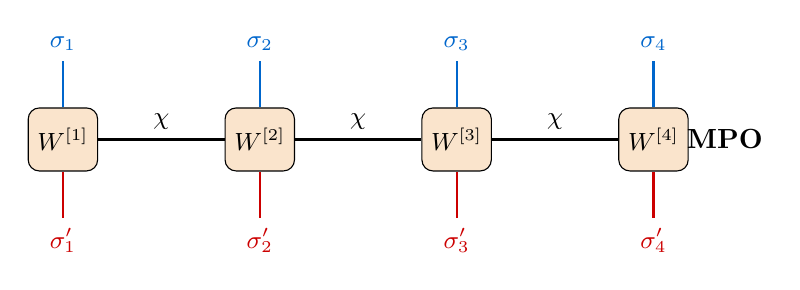
\begin{tikzpicture}[scale=1.0]
  \node[draw, rectangle, fill=myorange!20, minimum size=0.8cm, rounded corners] (w1) at (0,0) {\small$W^{[1]}$};
  \node[draw, rectangle, fill=myorange!20, minimum size=0.8cm, rounded corners] (w2) at (2.5,0) {\small$W^{[2]}$};
  \node[draw, rectangle, fill=myorange!20, minimum size=0.8cm, rounded corners] (w3) at (5,0) {\small$W^{[3]}$};
  \node[draw, rectangle, fill=myorange!20, minimum size=0.8cm, rounded corners] (w4) at (7.5,0) {\small$W^{[4]}$};

  % Horizontal bonds (virtual)
  \draw[thick] (w1) -- (w2) node[midway,above]{\small$\chi$};
  \draw[thick] (w2) -- (w3) node[midway,above]{\small$\chi$};
  \draw[thick] (w3) -- (w4) node[midway,above]{\small$\chi$};

  % Up legs
  \draw[thick,myblue] (w1) -- ++(0,1) node[above]{\small$\sigma_1$};
  \draw[thick,myblue] (w2) -- ++(0,1) node[above]{\small$\sigma_2$};
  \draw[thick,myblue] (w3) -- ++(0,1) node[above]{\small$\sigma_3$};
  \draw[thick,myblue] (w4) -- ++(0,1) node[above]{\small$\sigma_4$};

  % Down legs
  \draw[thick,myred] (w1) -- ++(0,-1) node[below]{\small$\sigma'_1$};
  \draw[thick,myred] (w2) -- ++(0,-1) node[below]{\small$\sigma'_2$};
  \draw[thick,myred] (w3) -- ++(0,-1) node[below]{\small$\sigma'_3$};
  \draw[thick,myred] (w4) -- ++(0,-1) node[below]{\small$\sigma'_4$};

  \node[right=0.3cm] at (w4) {\textbf{MPO}};
\end{tikzpicture}
\end{center}

\begin{exbox}[MPS vs MPO 的区别]
\begin{center}
\begin{tabular}{lcc}
\toprule
& \textbf{MPS} & \textbf{MPO} \\
\midrule
物理腿数 & 1（朝上或朝下） & 2（上 + 下） \\
身份 & "态"（向量） & "算符"（矩阵） \\
中间张量形状 & $[\chi, d, \chi]$ & $[\chi, d, d, \chi]$（或 $[d, \chi, d, \chi]$） \\
类比 & 量子态 $|\Psi\rangle$ & 哈密顿量 $\hat{H}$ 或转移矩阵 \\
\bottomrule
\end{tabular}
\end{center}
\end{exbox}

\subsection{第 2、3 行作为 MPO}

在 $4\times 4$ N 皇后问题中，第 2 行和第 3 行各构成一个 MPO：

\begin{center}
\begin{tikzpicture}[scale=1.0]
  % Row 2 MPO
  \node[draw, rectangle, fill=myorange!20, minimum size=0.8cm, rounded corners] (t21) at (0,0) {\small$T_{2,1}$};
  \node[draw, rectangle, fill=myorange!20, minimum size=0.8cm, rounded corners] (t22) at (3,0) {\small$T_{2,2}$};
  \node[draw, rectangle, fill=myorange!20, minimum size=0.8cm, rounded corners] (t23) at (6,0) {\small$T_{2,3}$};
  \node[draw, rectangle, fill=myorange!20, minimum size=0.8cm, rounded corners] (t24) at (9,0) {\small$T_{2,4}$};

  % Horizontal bonds
  \draw[thick] (t21) -- (t22) node[midway,above]{\small$8$};
  \draw[thick] (t22) -- (t23) node[midway,above]{\small$8$};
  \draw[thick] (t23) -- (t24) node[midway,above]{\small$8$};

  % Up legs
  \draw[thick,myblue] (t21) -- ++(0,1) node[above]{\small$u{=}8$};
  \draw[thick,myblue] (t22) -- ++(0,1) node[above]{\small$u{=}8$};
  \draw[thick,myblue] (t23) -- ++(0,1) node[above]{\small$u{=}8$};
  \draw[thick,myblue] (t24) -- ++(0,1) node[above]{\small$u{=}2$};

  % Down legs
  \draw[thick,myred] (t21) -- ++(0,-1) node[below]{\small$d{=}8$};
  \draw[thick,myred] (t22) -- ++(0,-1) node[below]{\small$d{=}8$};
  \draw[thick,myred] (t23) -- ++(0,-1) node[below]{\small$d{=}8$};
  \draw[thick,myred] (t24) -- ++(0,-1) node[below]{\small$d{=}2$};

  \node at (11,0) {\textbf{第2行 MPO}};
\end{tikzpicture}
\end{center}

张量形状：
\begin{center}
\begin{tabular}{ccl}
\toprule
\textbf{格点} & \textbf{形状} & \textbf{指标含义} \\
\midrule
$T_{2,1}$ (EL) & $[8, 8, 8]$ & (上:8, 下:8, 右键:8) \\
$T_{2,2}$ (B) & $[8, 8, 8, 8]$ & (上:8, 左键:8, 下:8, 右键:8) \\
$T_{2,3}$ (B) & $[8, 8, 8, 8]$ & (上:8, 左键:8, 下:8, 右键:8) \\
$T_{2,4}$ (ER) & $[2, 8, 2]$ & (上:2, 左键:8, 下:2) \\
\bottomrule
\end{tabular}
\end{center}

\begin{warnbox}[注意左端和右端的不对称性]
\begin{itemize}
  \item 左端 $T_{2,1}$：没有左键（左边界），上下物理腿都是 8（要传完整的列+两对角线信息）
  \item 右端 $T_{2,4}$：没有右键（右边界），上下物理腿只有 2（右边缘只剩一条对角线信息）
  \item 这种不对称性来自于对角线在边界处的消失
\end{itemize}
\end{warnbox}


%=============================================================================
\section{核心操作：MPO 作用于 MPS}
%=============================================================================

这是整个方法最关键的步骤。我们将逐个格点详细展示这个过程。

\subsection{概览}

\begin{keybox}[MPO $\times$ MPS = 新的 MPS]
将一个 MPO "作用"在一个 MPS 上，就像矩阵乘以向量：
$$|\Psi'\rangle = \hat{O} |\Psi\rangle$$

图形上：把 MPO 叠在 MPS 上方，将 MPO 的下腿与 MPS 的上腿缩并：

\begin{center}
\begin{tikzpicture}[scale=0.9]
  % MPS
  \node[draw, circle, fill=myblue!20, minimum size=0.6cm] (m1) at (0,0) {};
  \node[draw, circle, fill=myblue!20, minimum size=0.6cm] (m2) at (2,0) {};
  \node[draw, circle, fill=myblue!20, minimum size=0.6cm] (m3) at (4,0) {};
  \node[draw, circle, fill=myblue!20, minimum size=0.6cm] (m4) at (6,0) {};
  \draw[thick] (m1)--(m2)--(m3)--(m4);
  \draw[thick,myred] (m1)--++(0,0.8);
  \draw[thick,myred] (m2)--++(0,0.8);
  \draw[thick,myred] (m3)--++(0,0.8);
  \draw[thick,myred] (m4)--++(0,0.8);
  \node[left] at (-0.5,0) {\small MPS};

  % MPO
  \node[draw, rectangle, fill=myorange!20, minimum size=0.6cm] (o1) at (0,1.5) {};
  \node[draw, rectangle, fill=myorange!20, minimum size=0.6cm] (o2) at (2,1.5) {};
  \node[draw, rectangle, fill=myorange!20, minimum size=0.6cm] (o3) at (4,1.5) {};
  \node[draw, rectangle, fill=myorange!20, minimum size=0.6cm] (o4) at (6,1.5) {};
  \draw[thick] (o1)--(o2)--(o3)--(o4);
  \draw[thick,myred] (o1)--++(0,-0.8);
  \draw[thick,myred] (o2)--++(0,-0.8);
  \draw[thick,myred] (o3)--++(0,-0.8);
  \draw[thick,myred] (o4)--++(0,-0.8);
  \draw[thick,myblue] (o1)--++(0,0.8);
  \draw[thick,myblue] (o2)--++(0,0.8);
  \draw[thick,myblue] (o3)--++(0,0.8);
  \draw[thick,myblue] (o4)--++(0,0.8);
  \node[left] at (-0.5,1.5) {\small MPO};

  % Arrow
  \draw[-{Stealth},very thick] (7.5,0.75) -- (9,0.75);

  % Result MPS
  \node[draw, circle, fill=mypurple!20, minimum size=0.6cm] (n1) at (10,0.75) {};
  \node[draw, circle, fill=mypurple!20, minimum size=0.6cm] (n2) at (12,0.75) {};
  \node[draw, circle, fill=mypurple!20, minimum size=0.6cm] (n3) at (14,0.75) {};
  \node[draw, circle, fill=mypurple!20, minimum size=0.6cm] (n4) at (16,0.75) {};
  \draw[very thick] (n1)--(n2)--(n3)--(n4);
  \draw[thick,myblue] (n1)--++(0,0.8);
  \draw[thick,myblue] (n2)--++(0,0.8);
  \draw[thick,myblue] (n3)--++(0,0.8);
  \draw[thick,myblue] (n4)--++(0,0.8);
  \node[left] at (9.5,0.75) {\small 新MPS};
\end{tikzpicture}
\end{center}

\textbf{关键变化}：新 MPS 的虚拟键维度 = MPO 虚拟键 $\times$ 旧 MPS 虚拟键。

这就是为什么键维度会\textbf{指数增长}！
\end{keybox}

\subsection{逐格点详解：uMPS 吸收第 2 行 MPO}

初始 uMPS 是第 1 行张量，MPO 是第 2 行张量。我们逐格点展示缩并过程。

\subsubsection{格点 $j=1$（左端点）}

\begin{center}
\begin{tikzpicture}[scale=1.0]
  % uMPS{1}
  \node[draw, rectangle, fill=myblue!20, minimum width=1.4cm, minimum height=0.8cm, rounded corners] (mps) at (0,2) {\small$T_{1,1}$};
  \node[right=0.1cm,myblue] at (mps.east) {\small$[8,4]$};
  \draw[thick,myred] (mps) -- ++(0,-0.8) node[midway,right]{\small$d{=}8$};
  \draw[thick] (mps) -- ++(2,0) node[right]{\small$r{=}4$};

  % MPO{1}
  \node[draw, rectangle, fill=myorange!20, minimum width=1.4cm, minimum height=0.8cm, rounded corners] (mpo) at (0,0) {\small$T_{2,1}$};
  \node[right=0.1cm,myorange] at (mpo.east) {\small$[8,8,8]$};
  \draw[thick,myblue] (mpo) -- ++(0,0.7) node[midway,right]{\small$u{=}8$};
  \draw[thick,myred] (mpo) -- ++(0,-0.8) node[below]{\small$d'{=}8$};
  \draw[thick] (mpo) -- ++(2,0) node[right]{\small$r'{=}8$};

  % Contraction annotation
  \draw[thick,decorate,decoration={brace,amplitude=5pt}] (-1.5,0.75) -- (-1.5,1.15) node[midway,left=5pt]{\small\color{myred}缩并!};
\end{tikzpicture}
\end{center}

\textbf{操作}：将 MPO 的上腿 $u$（维度 8）与 MPS 的下腿 $d$（维度 8）缩并。

$$\text{新}M^{[1]}_{d',\;(r',r)} = \sum_{\alpha=1}^{8} T_{2,1}(\alpha, d', r') \cdot T_{1,1}(\alpha, r)$$

\begin{itemize}
  \item 缩并掉的指标：上-下连接（维度 8）
  \item 剩余指标：$d'$（新的下腿，维度 8）、$r'$（MPO 的右键，维度 8）、$r$（MPS 的右键，维度 4）
  \item 中间结果形状：$[8, 8, 4]$
  \item \textbf{Reshape}：将 $r'$ 和 $r$ 合并为一个右键 → $[8, 32]$
\end{itemize}

\begin{sumbox}[新 uMPS\{1\} 的形状：$[8, 32]$]
\begin{itemize}
  \item 物理腿（朝下）：维度 8（不变，来自 MPO 的下腿）
  \item 右虚拟键：维度 $8 \times 4 = 32$（MPO 右键 $\times$ 旧 MPS 右键）
\end{itemize}
\end{sumbox}

\begin{exbox}[为什么右键变成了 32？]
直觉：新的 MPS 需要同时记住两层信息——
\begin{enumerate}
  \item 第 1 行内部传递的信息（原虚拟键 $\chi=4$）
  \item 第 2 行内部传递的信息（MPO 虚拟键 $\chi'=8$）
\end{enumerate}
两者独立，所以用张量积 $4 \times 8 = 32$ 来编码。

具体地，新右键的 32 个状态 $(\alpha, \beta)$ 中：
\begin{itemize}
  \item $\alpha \in \{1,\ldots,8\}$：第 2 行向右传递的攻击线状态
  \item $\beta \in \{1,\ldots,4\}$：第 1 行向右传递的对角线状态
\end{itemize}
\end{exbox}

\subsubsection{格点 $j=2$（中间点）}

\begin{center}
\begin{tikzpicture}[scale=1.0]
  % uMPS{2}
  \node[draw, rectangle, fill=myblue!20, minimum width=1.4cm, minimum height=0.8cm, rounded corners] (mps) at (0,2) {\small$T_{1,2}$};
  \node[above=0.1cm,myblue] at (mps.north) {\small$[4,8,4]$};
  \draw[thick] (mps) -- ++(-2,0) node[left]{\small$l{=}4$};
  \draw[thick,myred] (mps) -- ++(0,-0.8) node[midway,right]{\small$d{=}8$};
  \draw[thick] (mps) -- ++(2,0) node[right]{\small$r{=}4$};

  % MPO{2}
  \node[draw, rectangle, fill=myorange!20, minimum width=1.4cm, minimum height=0.8cm, rounded corners] (mpo) at (0,0) {\small$T_{2,2}$};
  \node[below=0.1cm,myorange] at (mpo.south east) {\small$[8,8,8,8]$};
  \draw[thick] (mpo) -- ++(-2,0) node[left]{\small$l'{=}8$};
  \draw[thick,myblue] (mpo) -- ++(0,0.7) node[midway,right]{\small$u{=}8$};
  \draw[thick,myred] (mpo) -- ++(0,-1.3) node[below]{\small$d'{=}8$};
  \draw[thick] (mpo) -- ++(2,0) node[right]{\small$r'{=}8$};

  \draw[thick,decorate,decoration={brace,amplitude=5pt}] (-1.5,0.75) -- (-1.5,1.15) node[midway,left=5pt]{\small\color{myred}缩并!};
\end{tikzpicture}
\end{center}

\textbf{操作}：MPO 的上腿 $u$（8）与 MPS 的下腿 $d$（8）缩并。

$$\text{新}M^{[2]}_{(l',l),\;d',\;(r',r)} = \sum_{\alpha=1}^{8} T_{2,2}(\alpha, l', d', r') \cdot T_{1,2}(l, \alpha, r)$$

中间结果形状：$[8, 4, 8, 8, 4]$（分别对应 $l', l, d', r', r$）

Reshape：合并左键 $(l', l) \to 8\times 4 = 32$，合并右键 $(r', r) \to 8\times 4 = 32$

\begin{sumbox}[新 uMPS\{2\} 的形状：$[32, 8, 32]$]
\begin{itemize}
  \item 左虚拟键：$32 = 8 \times 4$
  \item 物理腿（朝下）：$8$
  \item 右虚拟键：$32 = 8 \times 4$
\end{itemize}
\end{sumbox}

\subsubsection{格点 $j=3$（同 $j=2$）}

完全相同的操作。新 uMPS\{3\}：$[32, 8, 32]$。

\subsubsection{格点 $j=4$（右端点）}

\begin{center}
\begin{tikzpicture}[scale=1.0]
  % uMPS{4}
  \node[draw, rectangle, fill=myblue!20, minimum width=1.4cm, minimum height=0.8cm, rounded corners] (mps) at (0,2) {\small$T_{1,4}$};
  \node[above=0.1cm,myblue] at (mps.north) {\small$[4,2]$};
  \draw[thick] (mps) -- ++(-2,0) node[left]{\small$l{=}4$};
  \draw[thick,myred] (mps) -- ++(0,-0.8) node[midway,right]{\small$d{=}2$};

  % MPO{4}
  \node[draw, rectangle, fill=myorange!20, minimum width=1.4cm, minimum height=0.8cm, rounded corners] (mpo) at (0,0) {\small$T_{2,4}$};
  \node[below=0.1cm,myorange] at (mpo.south east) {\small$[2,8,2]$};
  \draw[thick] (mpo) -- ++(-2,0) node[left]{\small$l'{=}8$};
  \draw[thick,myblue] (mpo) -- ++(0,0.7) node[midway,right]{\small$u{=}2$};
  \draw[thick,myred] (mpo) -- ++(0,-1.3) node[below]{\small$d'{=}2$};

  \draw[thick,decorate,decoration={brace,amplitude=5pt}] (-1.5,0.75) -- (-1.5,1.15) node[midway,left=5pt]{\small\color{myred}缩并!};
\end{tikzpicture}
\end{center}

注意这里 $u=d=2$，因为右边界只有一条对角线！

中间结果：$[8, 4, 2]$（$l', l, d'$） → Reshape 左键 → $[32, 2]$

\begin{sumbox}[新 uMPS\{4\} 的形状：$[32, 2]$]
\begin{itemize}
  \item 左虚拟键：$32 = 8 \times 4$
  \item 物理腿（朝下）：$2$
\end{itemize}
\end{sumbox}

\subsection{吸收后的 uMPS 全貌}

\begin{center}
\begin{tikzpicture}[scale=1.0]
  \node[draw, rectangle, fill=mypurple!20, minimum width=1.2cm, minimum height=0.8cm, rounded corners] (m1) at (0,0) {\small$M^{[1]}$};
  \node[draw, rectangle, fill=mypurple!20, minimum width=1.2cm, minimum height=0.8cm, rounded corners] (m2) at (3,0) {\small$M^{[2]}$};
  \node[draw, rectangle, fill=mypurple!20, minimum width=1.2cm, minimum height=0.8cm, rounded corners] (m3) at (6,0) {\small$M^{[3]}$};
  \node[draw, rectangle, fill=mypurple!20, minimum width=1.2cm, minimum height=0.8cm, rounded corners] (m4) at (9,0) {\small$M^{[4]}$};

  \draw[very thick] (m1) -- (m2) node[midway,above]{\small$\mathbf{32}$};
  \draw[very thick] (m2) -- (m3) node[midway,above]{\small$\mathbf{32}$};
  \draw[very thick] (m3) -- (m4) node[midway,above]{\small$\mathbf{32}$};

  \draw[thick,myred] (m1) -- ++(0,-1) node[below]{\small$8$};
  \draw[thick,myred] (m2) -- ++(0,-1) node[below]{\small$8$};
  \draw[thick,myred] (m3) -- ++(0,-1) node[below]{\small$8$};
  \draw[thick,myred] (m4) -- ++(0,-1) node[below]{\small$2$};

  \node[above] at (4.5,0.5) {\textbf{吸收第2行后的 uMPS（编码第1-2行的信息）}};

  % Shapes
  \node[below=1.3cm,mypurple] at (m1) {\small$[8,32]$};
  \node[below=1.3cm,mypurple] at (m2) {\small$[32,8,32]$};
  \node[below=1.3cm,mypurple] at (m3) {\small$[32,8,32]$};
  \node[below=1.3cm,mypurple] at (m4) {\small$[32,2]$};
\end{tikzpicture}
\end{center}

\begin{warnbox}[键维度的指数增长]
\begin{center}
\begin{tabular}{ccc}
\toprule
\textbf{阶段} & \textbf{虚拟键维度 $\chi$} & \textbf{编码了几行} \\
\midrule
初始（第 1 行） & 4 & 1 行 \\
吸收第 2 行后 & $4 \times 8 = 32$ & 2 行 \\
若继续吸收第 3 行 & $32 \times 8 = 256$ & 3 行 \\
若继续... & $256 \times 8 = 2048$ & 4 行 \\
\bottomrule
\end{tabular}
\end{center}
每吸收一行，$\chi$ 乘以 MPO 的虚拟键维度。这就是为什么\textbf{精确计算只能处理中等大小的 N}——$\chi$ 指数增长！对于近似计算，可以在每步之后用 SVD 截断到固定的 $\chi_{\max}$。
\end{warnbox}


%=============================================================================
\section{下方 MPS 吸收 MPO（反方向）}
%=============================================================================

\subsection{dMPS 吸收第 3 行}

过程完全对称，只是方向相反：MPO 的\textbf{下腿}与 dMPS 的\textbf{上腿}缩并。

\begin{center}
\begin{tikzpicture}[scale=0.9]
  % MPO row 3
  \node[draw, rectangle, fill=myorange!20, minimum size=0.6cm, rounded corners] (o1) at (0,1.5) {};
  \node[draw, rectangle, fill=myorange!20, minimum size=0.6cm, rounded corners] (o2) at (2.5,1.5) {};
  \node[draw, rectangle, fill=myorange!20, minimum size=0.6cm, rounded corners] (o3) at (5,1.5) {};
  \node[draw, rectangle, fill=myorange!20, minimum size=0.6cm, rounded corners] (o4) at (7.5,1.5) {};
  \draw[thick] (o1)--(o2)--(o3)--(o4);
  \draw[thick,myblue] (o1)--++(0,0.8);
  \draw[thick,myblue] (o2)--++(0,0.8);
  \draw[thick,myblue] (o3)--++(0,0.8);
  \draw[thick,myblue] (o4)--++(0,0.8);
  \draw[thick,myred] (o1)--++(0,-0.8);
  \draw[thick,myred] (o2)--++(0,-0.8);
  \draw[thick,myred] (o3)--++(0,-0.8);
  \draw[thick,myred] (o4)--++(0,-0.8);
  \node[left] at (-0.5,1.5) {\small 第3行MPO};

  % dMPS row 4
  \node[draw, rectangle, fill=mygreen!20, minimum size=0.6cm, rounded corners] (m1) at (0,0) {};
  \node[draw, rectangle, fill=mygreen!20, minimum size=0.6cm, rounded corners] (m2) at (2.5,0) {};
  \node[draw, rectangle, fill=mygreen!20, minimum size=0.6cm, rounded corners] (m3) at (5,0) {};
  \node[draw, rectangle, fill=mygreen!20, minimum size=0.6cm, rounded corners] (m4) at (7.5,0) {};
  \draw[thick] (m1)--(m2)--(m3)--(m4);
  \draw[thick,myred] (m1)--++(0,0.8);
  \draw[thick,myred] (m2)--++(0,0.8);
  \draw[thick,myred] (m3)--++(0,0.8);
  \draw[thick,myred] (m4)--++(0,0.8);
  \node[left] at (-0.5,0) {\small 第4行dMPS};

  % Arrow
  \draw[-{Stealth},very thick] (9,0.75) -- (10.5,0.75);

  % Result
  \node[draw, rectangle, fill=mypurple!20, minimum size=0.6cm, rounded corners] (n1) at (11.5,0.75) {};
  \node[draw, rectangle, fill=mypurple!20, minimum size=0.6cm, rounded corners] (n2) at (14,0.75) {};
  \node[draw, rectangle, fill=mypurple!20, minimum size=0.6cm, rounded corners] (n3) at (16.5,0.75) {};
  \draw[thick] (n1)--(n2)--(n3);
  \draw[thick,myblue] (n1)--++(0,0.8);
  \draw[thick,myblue] (n2)--++(0,0.8);
  \draw[thick,myblue] (n3)--++(0,0.8);
  \node[right] at (17.2,0.75) {\small 新dMPS};
  \node[right] at (11,0.75) {\small ...};
\end{tikzpicture}
\end{center}

以 $j=1$ 为例：
$$\text{新}D^{[1]}_{u',\;(r',r)} = \sum_{\alpha=1}^{8} T_{3,1}(u', \alpha, r') \cdot T_{4,1}(\alpha, r)$$

这里 $T_{3,1}$ 的\textbf{下腿} $d=\alpha$ 与 $T_{4,1}$ 的\textbf{上腿} $u=\alpha$ 缩并。

结果与上方完全对称：

\begin{center}
\begin{tabular}{ccc}
\toprule
\textbf{格点} & \textbf{新 dMPS 形状} & \textbf{指标} \\
\midrule
$j=1$ & $[8, 32]$ & (物理腿$u$:8, 右键:32) \\
$j=2$ & $[8, 32, 32]$ & (物理腿$u$:8, 左键:32, 右键:32) \\
$j=3$ & $[8, 32, 32]$ & (物理腿$u$:8, 左键:32, 右键:32) \\
$j=4$ & $[2, 32]$ & (物理腿$u$:2, 左键:32) \\
\bottomrule
\end{tabular}
\end{center}


%=============================================================================
\section{最终缩并：两个 MPS 的内积}
%=============================================================================

\subsection{全局图景}

现在我们有两个 MPS 在第 2-3 行之间对接：

\begin{center}
\begin{tikzpicture}[scale=1.0]
  % uMPS
  \node[draw, rectangle, fill=myblue!30, minimum width=1cm, minimum height=0.7cm, rounded corners] (u1) at (0,1) {\tiny$[8,32]$};
  \node[draw, rectangle, fill=myblue!30, minimum width=1cm, minimum height=0.7cm, rounded corners] (u2) at (3,1) {\tiny$[32,8,32]$};
  \node[draw, rectangle, fill=myblue!30, minimum width=1cm, minimum height=0.7cm, rounded corners] (u3) at (6,1) {\tiny$[32,8,32]$};
  \node[draw, rectangle, fill=myblue!30, minimum width=1cm, minimum height=0.7cm, rounded corners] (u4) at (9,1) {\tiny$[32,2]$};
  \draw[very thick] (u1)--(u2) node[midway,above]{\small$32$};
  \draw[very thick] (u2)--(u3) node[midway,above]{\small$32$};
  \draw[very thick] (u3)--(u4) node[midway,above]{\small$32$};

  % dMPS
  \node[draw, rectangle, fill=mygreen!30, minimum width=1cm, minimum height=0.7cm, rounded corners] (d1) at (0,-1) {\tiny$[8,32]$};
  \node[draw, rectangle, fill=mygreen!30, minimum width=1cm, minimum height=0.7cm, rounded corners] (d2) at (3,-1) {\tiny$[8,32,32]$};
  \node[draw, rectangle, fill=mygreen!30, minimum width=1cm, minimum height=0.7cm, rounded corners] (d3) at (6,-1) {\tiny$[8,32,32]$};
  \node[draw, rectangle, fill=mygreen!30, minimum width=1cm, minimum height=0.7cm, rounded corners] (d4) at (9,-1) {\tiny$[2,32]$};
  \draw[very thick] (d1)--(d2) node[midway,below]{\small$32$};
  \draw[very thick] (d2)--(d3) node[midway,below]{\small$32$};
  \draw[very thick] (d3)--(d4) node[midway,below]{\small$32$};

  % Physical connections
  \draw[thick,myred] (u1)--(d1) node[midway,right]{\small$8$};
  \draw[thick,myred] (u2)--(d2) node[midway,right]{\small$8$};
  \draw[thick,myred] (u3)--(d3) node[midway,right]{\small$8$};
  \draw[thick,myred] (u4)--(d4) node[midway,right]{\small$2$};

  \node[above=0.3cm] at (u2.north) {\textbf{uMPS}（第1-2行）};
  \node[below=0.3cm] at (d2.south) {\textbf{dMPS}（第3-4行）};
  \node[right=0.3cm,myred] at (10,0) {物理腿对接};
\end{tikzpicture}
\end{center}

内积的计算 = 缩并所有红线（物理腿）和所有黑线（虚拟键），最终得到一个标量 $Z_4$。

\subsection{拉拉链式缩并}

不能一次全缩并（太贵了）。采用\textbf{从左到右逐列}的方式：

\subsubsection{第 1 列}

$$Z^{(1)}_{r_u, r_d} = \sum_{p_1=1}^{8} u^{[1]}_{p_1, r_u} \cdot d^{[1]}_{p_1, r_d}$$

\begin{center}
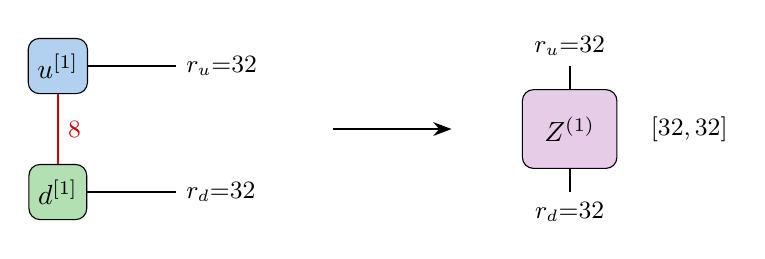
\begin{tikzpicture}[scale=1.0]
  \node[draw, rectangle, fill=myblue!30, minimum size=0.7cm, rounded corners] (u) at (0,0.8) {$u^{[1]}$};
  \node[draw, rectangle, fill=mygreen!30, minimum size=0.7cm, rounded corners] (d) at (0,-0.8) {$d^{[1]}$};
  \draw[thick,myred] (u)--(d) node[midway,right]{\small$8$};
  \draw[thick] (u)--++(1.5,0) node[right]{\small$r_u{=}32$};
  \draw[thick] (d)--++(1.5,0) node[right]{\small$r_d{=}32$};

  \draw[-{Stealth},thick] (3.5,0)--(5,0);

  \node[draw, rectangle, fill=mypurple!20, minimum width=1.2cm, minimum height=1cm, rounded corners] (z) at (6.5,0) {$Z^{(1)}$};
  \draw[thick] (z)--++(0,0.8) node[above]{\small$r_u{=}32$};
  \draw[thick] (z)--++(0,-0.8) node[below]{\small$r_d{=}32$};
  \node[right=0.3cm] at (z.east) {\small$[32,32]$};
\end{tikzpicture}
\end{center}

结果 $Z^{(1)}$ 是一个 $32 \times 32$ 的矩阵。

\subsubsection{第 2 列}

$$Z^{(2)}_{r_u, r_d} = \sum_{l_u, l_d, p} Z^{(1)}_{l_u, l_d} \cdot u^{[2]}_{l_u, p, r_u} \cdot d^{[2]}_{p, l_d, r_d}$$

\begin{center}
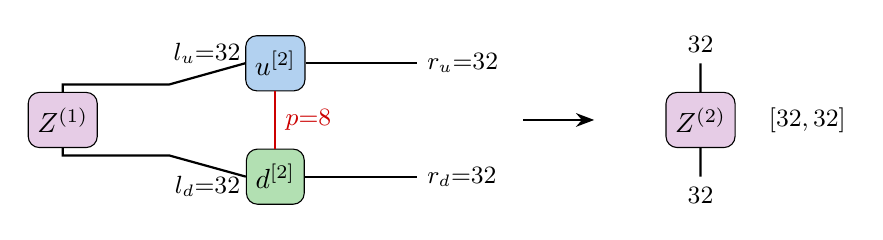
\begin{tikzpicture}[scale=0.9]
  % Z(1)
  \node[draw, rectangle, fill=mypurple!20, minimum size=0.7cm, rounded corners] (z) at (0,0) {$Z^{(1)}$};

  % u[2]
  \node[draw, rectangle, fill=myblue!30, minimum size=0.7cm, rounded corners] (u) at (3,0.8) {$u^{[2]}$};

  % d[2]
  \node[draw, rectangle, fill=mygreen!30, minimum size=0.7cm, rounded corners] (d) at (3,-0.8) {$d^{[2]}$};

  % Connections
  \draw[thick] (z)--++(0,0.5)--++(1.5,0)--(u.west) node[midway,above]{\small$l_u{=}32$};
  \draw[thick] (z)--++(0,-0.5)--++(1.5,0)--(d.west) node[midway,below]{\small$l_d{=}32$};
  \draw[thick,myred] (u)--(d) node[midway,right]{\small$p{=}8$};
  \draw[thick] (u)--++(2,0) node[right]{\small$r_u{=}32$};
  \draw[thick] (d)--++(2,0) node[right]{\small$r_d{=}32$};

  \draw[-{Stealth},thick] (6.5,0)--(7.5,0);

  \node[draw, rectangle, fill=mypurple!20, minimum size=0.7cm, rounded corners] (z2) at (9,0) {$Z^{(2)}$};
  \draw[thick] (z2)--++(0,0.8) node[above]{\small$32$};
  \draw[thick] (z2)--++(0,-0.8) node[below]{\small$32$};
  \node[right=0.3cm] at (z2.east) {\small$[32,32]$};
\end{tikzpicture}
\end{center}

关键：三个指标 $l_u$（32）、$l_d$（32）、$p$（8）全部被求和掉，只留下 $r_u$（32）和 $r_d$（32）。

\textbf{计算量}：$32 \times 32 \times 8 \times 32 \times 32 \approx 2.7 \times 10^7$ 次乘法。

\subsubsection{第 3 列：同第 2 列}

$Z^{(3)}$：形状 $[32, 32]$。

\subsubsection{第 4 列（最后一列）}

$$Z_4 = \sum_{l_u, l_d, p} Z^{(3)}_{l_u, l_d} \cdot u^{[4]}_{l_u, p} \cdot d^{[4]}_{p, l_d}$$

所有指标全部缩并 $\to$ 得到标量！

\begin{center}
\begin{tikzpicture}[scale=0.9]
  \node[draw, rectangle, fill=mypurple!20, minimum size=0.7cm, rounded corners] (z) at (0,0) {$Z^{(3)}$};
  \node[draw, rectangle, fill=myblue!30, minimum size=0.7cm, rounded corners] (u) at (3,0.8) {$u^{[4]}$};
  \node[draw, rectangle, fill=mygreen!30, minimum size=0.7cm, rounded corners] (d) at (3,-0.8) {$d^{[4]}$};
  \draw[thick] (z)--++(0,0.5)--++(1.5,0)--(u.west) node[midway,above]{\small$32$};
  \draw[thick] (z)--++(0,-0.5)--++(1.5,0)--(d.west) node[midway,below]{\small$32$};
  \draw[thick,myred] (u)--(d) node[midway,right]{\small$2$};

  \draw[-{Stealth},thick] (5.5,0)--(6.5,0);
  \node[draw, circle, fill=myorange!30, minimum size=1cm] (res) at (8,0) {\Large$\mathbf{2}$};
  \node[below=0.3cm] at (res.south) {标量 = $Z_4$};
\end{tikzpicture}
\end{center}

\begin{sumbox}[$Z_4 = 2$：4 皇后有 2 个解！]
这两个解分别是：
\begin{center}
\begin{tikzpicture}[scale=0.6]
  % Solution 1
  \draw[step=1] (0,0) grid (4,4);
  \fill[myblue!60] (1.5,3.5) circle(0.3);
  \fill[myblue!60] (3.5,2.5) circle(0.3);
  \fill[myblue!60] (0.5,1.5) circle(0.3);
  \fill[myblue!60] (2.5,0.5) circle(0.3);
  \node at (2,-0.5) {解 1};

  % Solution 2
  \begin{scope}[xshift=6cm]
  \draw[step=1] (0,0) grid (4,4);
  \fill[myblue!60] (2.5,3.5) circle(0.3);
  \fill[myblue!60] (0.5,2.5) circle(0.3);
  \fill[myblue!60] (3.5,1.5) circle(0.3);
  \fill[myblue!60] (1.5,0.5) circle(0.3);
  \node at (2,-0.5) {解 2};
  \end{scope}
\end{tikzpicture}
\end{center}
\end{sumbox}


%=============================================================================
\section{完整流程总结}
%=============================================================================

\begin{center}
\begin{tikzpicture}[scale=0.8, every node/.style={font=\small}]
  % Step 1
  \node[draw, rectangle, fill=lightyellow, minimum width=3cm, minimum height=1cm, rounded corners] (s1) at (0,4) {第1行 → uMPS};
  \node[draw, rectangle, fill=lightyellow, minimum width=3cm, minimum height=1cm, rounded corners] (s2) at (0,2) {第4行 → dMPS};

  % Step 2
  \node[draw, rectangle, fill=lightblue, minimum width=4cm, minimum height=1cm, rounded corners] (s3) at (7,4) {uMPS 吸收第2行 MPO};
  \node[draw, rectangle, fill=lightblue, minimum width=4cm, minimum height=1cm, rounded corners] (s4) at (7,2) {dMPS 吸收第3行 MPO};

  % Step 3
  \node[draw, rectangle, fill=lightgreen, minimum width=4cm, minimum height=1.2cm, rounded corners] (s5) at (14,3) {uMPS 与 dMPS 内积};

  % Result
  \node[draw, circle, fill=lightred, minimum size=1.5cm] (res) at (14,0.5) {\Large$Z_N$};

  \draw[-{Stealth},thick] (s1)--(s3);
  \draw[-{Stealth},thick] (s2)--(s4);
  \draw[-{Stealth},thick] (s3)--(s5);
  \draw[-{Stealth},thick] (s4)--(s5);
  \draw[-{Stealth},thick] (s5)--(res);

  % Annotations
  \node[below=0.1cm,gray] at (s1.south) {$\chi = 4$};
  \node[below=0.1cm,gray] at (s2.south) {$\chi = 4$};
  \node[below=0.1cm,gray] at (s3.south) {$\chi = 32$};
  \node[below=0.1cm,gray] at (s4.south) {$\chi = 32$};
\end{tikzpicture}
\end{center}

\begin{keybox}[为什么从两头往中间缩并？]
如果只从上往下，缩并 $N-1$ 行 MPO 后 $\chi = 4 \times 8^{N-2}$。

从两头往中间，各只缩并 $\sim N/2$ 行，最大 $\chi \approx 4 \times 8^{N/2-1}$，指数减半！

对于 $N=8$：
\begin{itemize}
  \item 单方向：$\chi_{\max} = 4 \times 8^6 = 1{,}048{,}576$
  \item 双方向：$\chi_{\max} = 4 \times 8^2 = 256$（快了 $4096$ 倍！）
\end{itemize}
\end{keybox}

\subsection{计算复杂度}

对于 $N \times N$ 的棋盘：
\begin{itemize}
  \item MPO 虚拟键维度 $D = 8$
  \item 吸收 $k$ 行后 MPS 虚拟键 $\chi_k \sim 4 \times 8^{k-1}$（精确缩并，不截断）
  \item 总计算量主导项：$O(N \cdot \chi_{\max}^2 \cdot D^2)$
  \item 最大 $\chi \approx 4 \times 8^{N/2-1}$，所以复杂度 $\sim O(N \cdot 8^N)$
\end{itemize}

虽然仍是指数级，但比暴力枚举 $2^{N^2}$ 好得多（暴力需要检查所有格子的所有占据方式）。

\subsection{如何拓展到更大的 N？}

\begin{keybox}[近似方法：SVD 截断]
在每次 MPO 吸收后，对新 MPS 做 SVD 分解，只保留最大的 $\chi_{\max}$ 个奇异值：

$$M^{[j]} \approx U \cdot S \cdot V^\dagger \quad \text{（只保留前 $\chi_{\max}$ 个）}$$

这样虚拟键维度被控制在 $\chi_{\max}$，但会引入近似误差。$\chi_{\max}$ 越大越精确。

当前代码没有做截断（精确计算），所以只能算到 $N \sim 20$。
\end{keybox}


%=============================================================================
\section{附录：所有张量的详细形状一览}
%=============================================================================

\subsection{$4 \times 4$ 所有格点张量}

\begin{center}
\renewcommand{\arraystretch}{1.5}
\begin{tabular}{c|c|c|c|c}
\toprule
& $j=1$ & $j=2$ & $j=3$ & $j=4$ \\
\midrule
$i=1$ & $T_{1,1}$: $[8,4]$ & $T_{1,2}$: $[4,8,4]$ & $T_{1,3}$: $[4,8,4]$ & $T_{1,4}$: $[4,2]$ \\
& (CLU) & (EU) & (EU) & (CRU) \\
& $(d,r)$ & $(l,d,r)$ & $(l,d,r)$ & $(l,d)$ \\
\midrule
$i=2$ & $T_{2,1}$: $[8,8,8]$ & $T_{2,2}$: $[8,8,8,8]$ & $T_{2,3}$: $[8,8,8,8]$ & $T_{2,4}$: $[2,8,2]$ \\
& (EL) & (B) & (B) & (ER) \\
& $(u,d,r)$ & $(u,l,d,r)$ & $(u,l,d,r)$ & $(u,l,d)$ \\
\midrule
$i=3$ & $T_{3,1}$: $[8,8,8]$ & $T_{3,2}$: $[8,8,8,8]$ & $T_{3,3}$: $[8,8,8,8]$ & $T_{3,4}$: $[2,8,2]$ \\
& (EL) & (B) & (B) & (ER) \\
& $(u,d,r)$ & $(u,l,d,r)$ & $(u,l,d,r)$ & $(u,l,d)$ \\
\midrule
$i=4$ & $T_{4,1}$: $[8,4]$ & $T_{4,2}$: $[8,4,4]$ & $T_{4,3}$: $[8,4,4]$ & $T_{4,4}$: $[2,4]$ \\
& (CLD) & (ED) & (ED) & (CRD) \\
& $(u,r)$ & $(u,l,r)$ & $(u,l,r)$ & $(u,l)$ \\
\bottomrule
\end{tabular}
\end{center}

\subsection{缩并过程中的 MPS 形状变化}

\begin{center}
\renewcommand{\arraystretch}{1.5}
\begin{tabular}{c|c|c|c|c}
\toprule
\textbf{阶段} & $j=1$ & $j=2$ & $j=3$ & $j=4$ \\
\midrule
初始 uMPS (第1行) & $[8,4]$ & $[4,8,4]$ & $[4,8,4]$ & $[4,2]$ \\
吸收第2行后 & $[8,\mathbf{32}]$ & $[\mathbf{32},8,\mathbf{32}]$ & $[\mathbf{32},8,\mathbf{32}]$ & $[\mathbf{32},2]$ \\
\midrule
初始 dMPS (第4行) & $[8,4]$ & $[8,4,4]$ & $[8,4,4]$ & $[2,4]$ \\
吸收第3行后 & $[8,\mathbf{32}]$ & $[8,\mathbf{32},\mathbf{32}]$ & $[8,\mathbf{32},\mathbf{32}]$ & $[2,\mathbf{32}]$ \\
\midrule
内积 $Z^{(j)}$ & $[32,32]$ & $[32,32]$ & $[32,32]$ & $\mathbf{2}$（标量） \\
\bottomrule
\end{tabular}
\end{center}


%=============================================================================
\section{直觉总结}
%=============================================================================

\begin{sumbox}[一句话理解整个方法]
\textbf{将 2D 棋盘按行切成 1D 条带}：
\begin{enumerate}
  \item 每一行是一个 MPS 或 MPO
  \item 将 MPO 逐行"压"进 MPS（类似矩阵乘向量）
  \item 最终两个 MPS 做内积 → 得到合法配置数
\end{enumerate}

键维度 $\chi$ 的增长反映了\textbf{跨行纠缠/关联}的复杂度——需要记住多少关于上方/下方行的信息。
\end{sumbox}

\begin{sumbox}[类比：为什么叫"矩阵乘积"？]
回想 1D 系统的配分函数：
$$Z = \text{Tr}(T^N) = \text{Tr}(T \cdot T \cdot T \cdots T)$$
这就是一连串矩阵乘法（转移矩阵法）。

MPS/MPO 方法是它的\textbf{2D 推广}：
\begin{itemize}
  \item 1D 的转移矩阵 $T$ → 2D 的 MPO（矩阵变成了矩阵的"链"）
  \item 1D 的 $\text{Tr}$ → 2D 的 MPS 内积
  \item 1D 的 $T^N$ → 2D 的逐行 MPO 吸收
\end{itemize}
\end{sumbox}

\end{document}
